% FedPASA @ WWW'27 — double-blind submission draft
% Build: powershell -ExecutionPolicy Bypass -File build.ps1
\documentclass[sigconf,anonymous,balance=false]{acmart}

\usepackage{amsmath}
\usepackage{amsthm}
\usepackage{booktabs}
\usepackage{multirow}
\usepackage{graphicx}
\usepackage{algorithm}
\usepackage{algpseudocode}
\usepackage{tabularx}
\usepackage{xcolor}
\usepackage{colortbl}
\usepackage{needspace}
\setlength{\emergencystretch}{1em}
\setlength{\textfloatsep}{10pt plus 2pt minus 2pt}
\setlength{\dbltextfloatsep}{10pt plus 2pt minus 2pt}
\setlength{\floatsep}{8pt plus 2pt minus 2pt}
\renewcommand{\topfraction}{0.9}
\renewcommand{\dbltopfraction}{0.95}
\renewcommand{\textfraction}{0.08}
\renewcommand{\floatpagefraction}{0.85}

\newtheorem{proposition}{Proposition}

\setcopyright{none}
\settopmatter{printacmref=true,printfolios=true}
\acmConference[WWW '27]{The ACM Web Conference 2027}{May 10--14, 2027}{Dublin, Ireland}
\acmBooktitle{Proceedings of the ACM Web Conference 2027 (WWW '27)}
\acmYear{2027}
\copyrightyear{2027}
\acmDOI{}
\acmISBN{}

\begin{document}
\raggedbottom

\title{FedPASA: Reliability-Aware Semantic Adaptation for Cross-Domain Federated Recommendation}

\author{Anonymous Author(s)}


\begin{abstract}
Federated recommendation (FR) enables collaborative model training while keeping user interactions local. However, transferring recommendation knowledge across services remains challenging due to disjoint item catalogs and uneven target-domain supervision. Frequently observed items provide abundant interaction evidence, whereas low-frequency items offer limited supervision, and client-specific preferences further introduce heterogeneity into semantic adaptation. Existing approaches commonly employ shared transformations or client-level personalization without explicitly accounting for differences in item-level supervision. To address these challenges, we propose FedPASA, a reliability-aware semantic adaptation framework for cross-domain federated recommendation. FedPASA introduces Popularity-Gated Dual-path Routing (PGDR), which combines two residual adaptation paths using item-frequency-derived weights. A private client profile further conditions the adapted representations through feature-wise scaling and shifting, while AutoAnchor incorporates pretrained semantic information through catalog-level anchoring. Extensive experiments on real-world cross-domain recommendation benchmarks demonstrate the effectiveness of FedPASA. The proposed framework achieves superior average cross-domain recommendation performance over competitive baselines under both sampled and full-catalog ranking. Further analyses demonstrate that frequency-aware routing improves recommendation accuracy beyond additional adapter capacity, while client conditioning and semantic anchoring provide complementary adaptation capabilities.
\end{abstract}


\begin{CCSXML}
<ccs2012>
<concept><concept_id>10002951.10003317.10003347.10003350</concept_id>
<concept_desc>Information systems~Recommender systems</concept_desc>
<concept_significance>500</concept_significance></concept>
<concept><concept_id>10010147.10010919</concept_id>
<concept_desc>Computing methodologies~Distributed computing methodologies</concept_desc>
<concept_significance>300</concept_significance></concept>
</ccs2012>
\end{CCSXML}
\ccsdesc[500]{Information systems~Recommender systems}
\ccsdesc[300]{Computing methodologies~Distributed computing methodologies}

\keywords{Federated Recommendation; Cross-Domain Recommendation; Semantic Transfer; Long-tail Recommendation}

\maketitle

% !TeX root = ../main.tex
\section{Introduction}
\label{sec:intro}
With the growth of e-commerce and digital services, recommender systems have become essential infrastructure for online platforms. However, traditional recommender systems typically consolidate vast amounts of user data centrally, leading to privacy and regulatory concerns. Federated learning allows multiple clients to collaboratively train a model without sharing raw data; federated recommendation (FR) applies this idea to recommendation, where interaction histories remain on local devices and only model parameters are aggregated~\citep{ammad2019federated,mcmahan2017communication}.

Meanwhile, cross-domain transfer is another longstanding need: platforms wish to reuse a mature catalog to bootstrap a new service, where newly listed items lack behavioral evidence. However, existing cross-domain recommenders typically assume overlapping users or alignable item identifiers, and neither premise holds under federated constraints---participating services cannot pool user histories, and disjoint catalogs share no identifiers to align. We study this disjoint-catalog setting without requiring linked users between source and target domains.

A viable route is offered by pretrained text encoders: items from different catalogs are mapped into a common semantic space, enabling transfer without matching identifiers~\citep{zhang2026transfr}. However, the semantic space alone does not resolve the uneven supervision of the target domain. On the one hand, frequently observed items supply many ranking constraints, whereas rare items provide little evidence for adaptation; on the other hand, clients observe different semantic regions through their own histories, so a globally rare item may be familiar to one client yet unseen by another. Moreover, excessive adaptation drifts representations away from the pretrained semantics, harming items with scarce evidence. An adaptation rule therefore needs to account for the amount of item-level evidence, the client context in which it is observed, and how much of the pretrained prior should be preserved.

Personalized adapters and expert mixtures address variation across clients~\citep{li2026fedvlr,li2026fedpa}, but client-level personalization does not by itself specify how items with different training frequencies should share adaptation paths: a single shared transformation applies the same parameterization to all items, and an additional adapter introduces capacity without determining how to allocate it. In this light, we use item frequency as an observable proxy for the available target supervision, route each item between two residual paths, and adjust the routed representation to the local interaction profile through client conditioning.

To address the challenges mentioned above, we propose FedPASA, which combines three operations in a shared semantic adapter. Specifically, Popularity-Gated Dual-path Routing (PGDR) mixes a source-initialized path and a target-initialized path using a frequency-derived weight; client conditioning produces feature-wise scales and shifts from a locally pooled semantic profile; in addition, AutoAnchor interpolates the resulting representation with the frozen text embedding, with the anchor strength set by a catalog-level user-to-item ratio. Both residual paths are updated on the target domain, while source initialization provides a starting point rather than a fixed representation.

We evaluate this design on multiple real-world datasets, with controls that separate frequency assignment, model capacity, and final personalization. Our contributions are summarized as follows:
\begin{itemize}
\item We propose FedPASA, a reliability-aware semantic adaptation framework that adjusts item representations according to evidence strength at the item, client, and catalog levels. Our framework is motivated by an analysis of the failure of uniform adaptation in existing federated semantic transfer methods under uneven target supervision: a single shared transformation underfits well-supported frequent items while overfitting sparsely observed items. The proposed framework applies to different backbone encoders.
\item We design PGDR to combine two trainable residual adaptation paths using frequency-derived weights, without an additional learned routing network. Client conditioning adjusts the combined representations using local semantic profiles, while AutoAnchor controls their mixture with the frozen semantic prior through a catalog-level rule.
\item We conduct extensive experiments on multiple real-world datasets. With the same text encoder, FedPASA achieves higher average cross-domain recommendation accuracy than the evaluated baselines. Comparisons that retain the same network structure and parameter count further show that frequency-derived mixing weights outperform using a common pair of weights for all items or shuffling the item--weight assignments. Ablation studies further characterize the effects of individual components.
\end{itemize}

\par\addvspace{6pt}\noindent\begin{minipage}{\columnwidth}
\centering
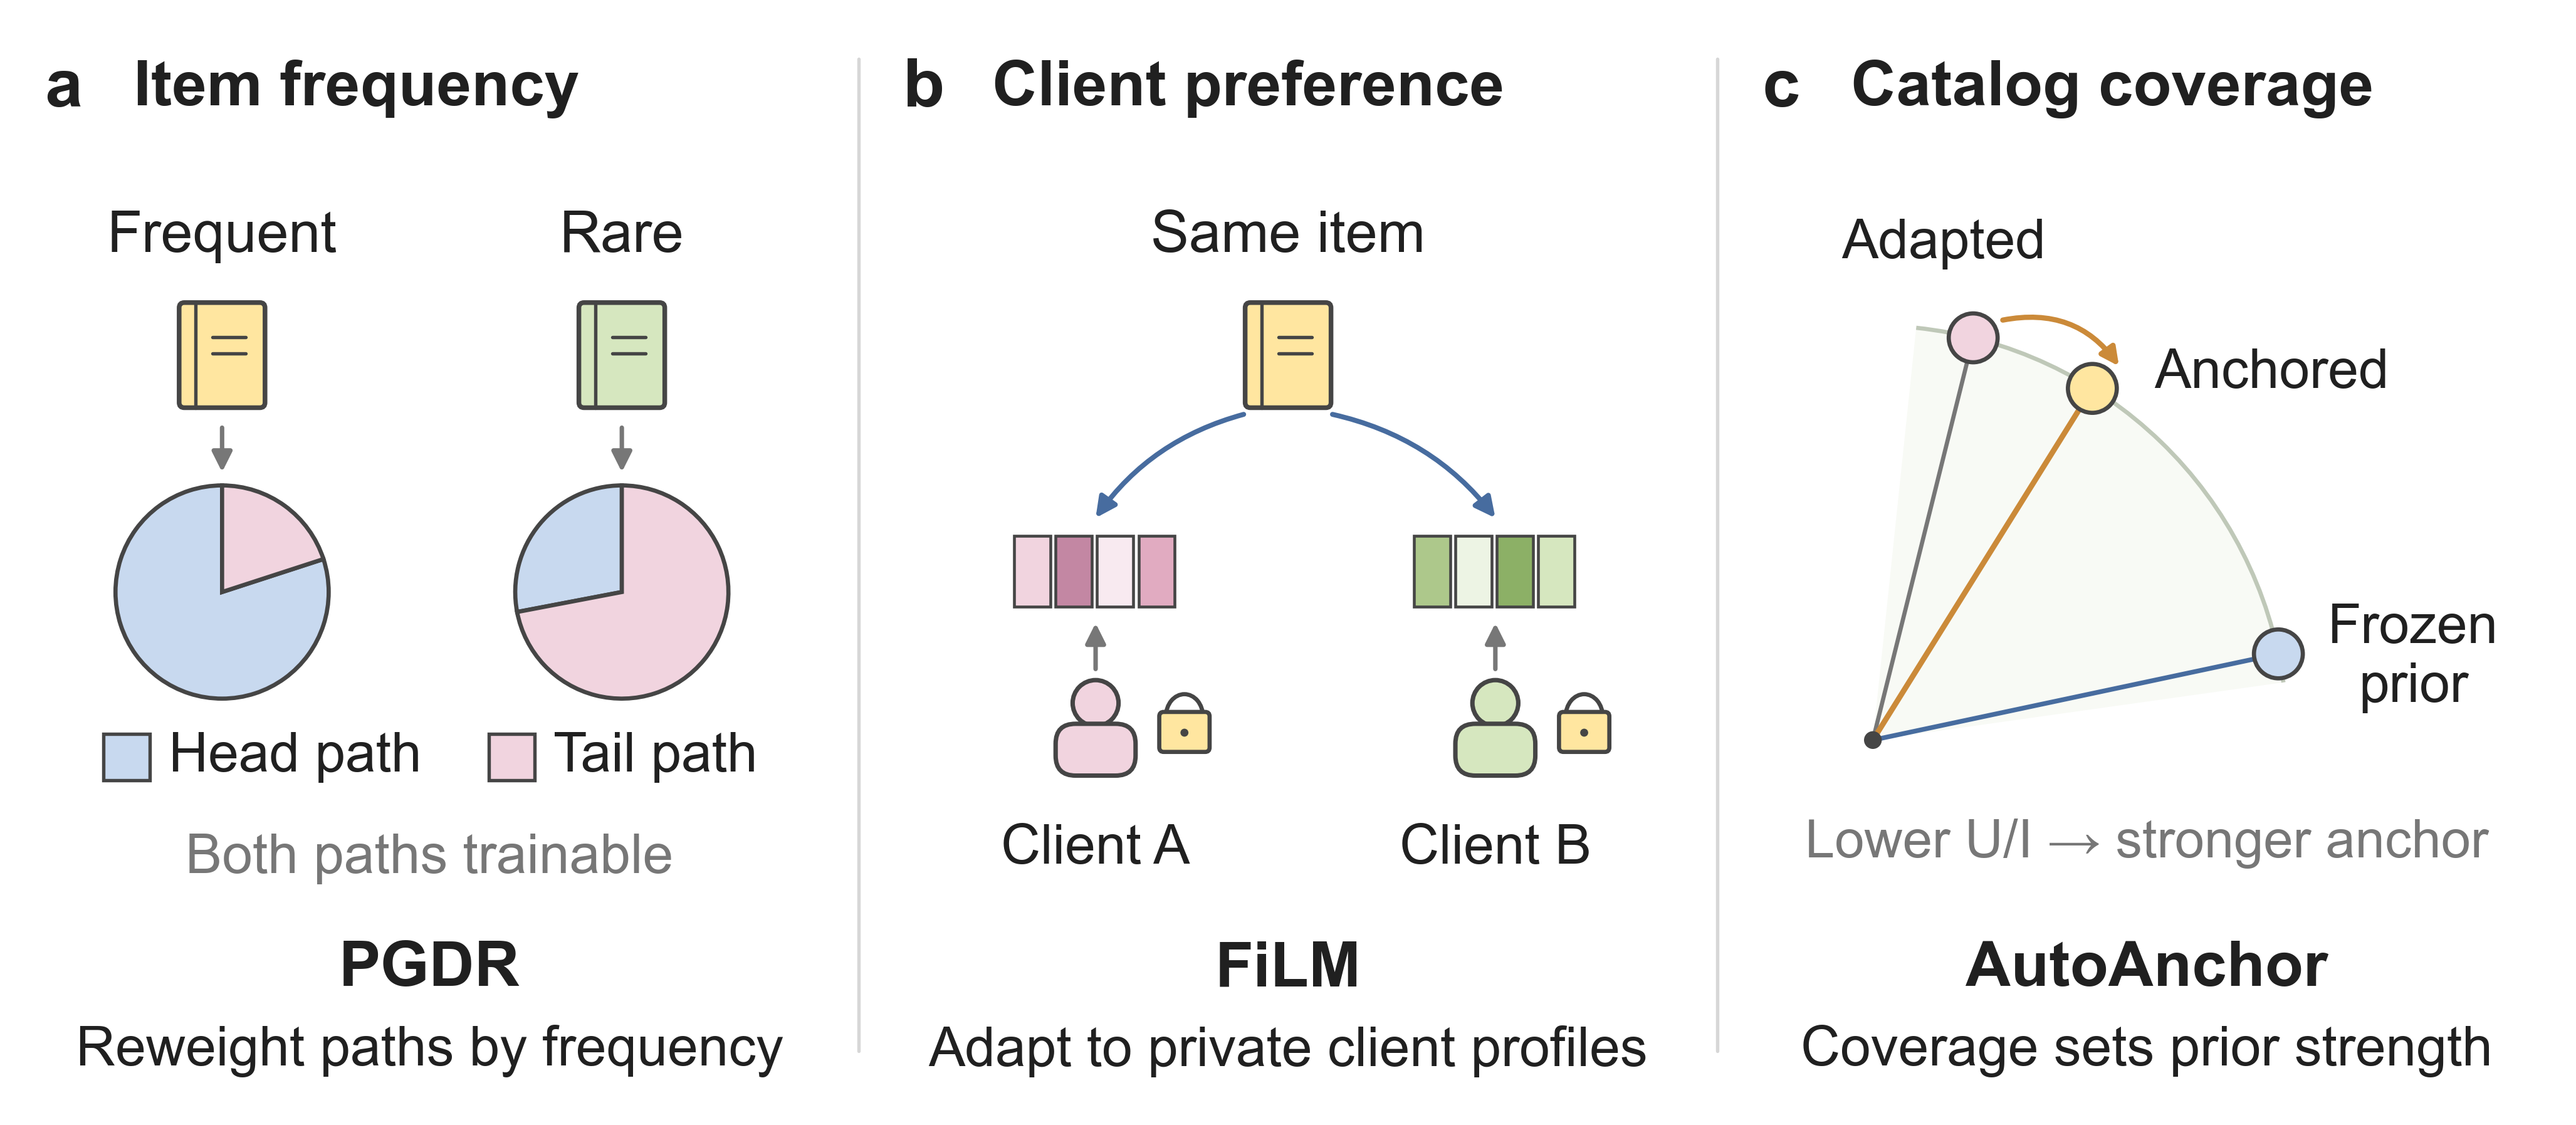
\includegraphics[width=\linewidth]{figures/adaptation_overview.png}
\captionof{figure}{Three adaptation controls: (a) frequency-based path mixing; (b) private-profile conditioning; (c) catalog-dependent prior preservation.}
\label{fig:adaptation-overview}
\end{minipage}\par\addvspace{6pt}


% !TeX root = ../main.tex
\section{Related Work}
\label{sec:related}
\subsection{Federated Semantic Transfer}
FR learns shared parameters from decentralized interactions~\citep{ammad2019federated,mcmahan2017communication}; proximal optimization and local components address heterogeneity~\citep{li2020federated,arivazhagan2019federated,dinh2020personalized,li2021ditto}. Transferring item-ID models across disjoint catalogs requires alignment or content. TransFR combines pretrained language representations, adapter tuning, and local personalization~\citep{zhang2026transfr}. FedDCSR disentangles shared and domain-specific sequential factors~\citep{zhang2024feddcsr}; PFCR and FFMSR transfer text-derived content~\citep{guo2024pfcr,lu2025ffmsr}; FedCRF uses semantic graphs and contrastive fusion~\citep{guo2026fedcrf}. FeDecider personalizes LoRA aggregation with client-specific directional weights~\citep{he2026fedecider}. Beyond sequence modeling, fusion, and aggregation, FedPASA studies item-level supervision allocation within a shared semantic adapter.

\subsection{Personalization and Preservation}
FedPA combines private user adapters, shared group adapters, and adaptive gating~\citep{li2026fedpa}; FedVLR personalizes multimodal expert mixtures~\citep{li2026fedvlr}. ESAM addresses long-tail imbalance~\citep{chen2021esam}, MeLU adapts user preferences~\citep{lee2019melu}, and multi-gate MoE learns input-dependent expert combinations~\citep{ma2018mmoe}. PGDR instead derives deterministic routing weights from target item frequency. Learned, constant, and shuffled routing provide comparisons that isolate this allocation rule.

FiLM applies feature-wise scales and shifts~\citep{perez2018film}; FedPASA generates them from a private client profile within a shared adapter. L2-SP and DELTA preserve source information through parameter or feature penalties~\citep{li2018explicit,li2019delta}. AutoAnchor instead interpolates the normalized ranking representation with the frozen semantic prior. Its fixed catalog-level coverage heuristic is motivated by bias--variance and geometric analyses and assessed through ranking experiments.


% !TeX root = ../main.tex
\section{FedPASA}
\label{sec:method}

\subsection{Problem Setup and Overview}
\label{sec:setup}

We consider cross-domain federated recommendation with disjoint item catalogs. Let $\mathcal{C}$, $\mathcal{U}$, and $\mathcal{I}$ denote the sets of clients, users, and target items, respectively. Each client $c$ maintains a subset of users $\mathcal{U}_c$ and their interaction histories locally. A frozen text encoder maps each item $i$ to a unit-normalized semantic representation $x_i\in\mathbb{R}^d$, providing a common representation space across domains. Each user $u$ is associated with a private embedding $e_u\in\mathbb{R}^d$ that remains on its corresponding client.

FedPASA adapts the frozen semantic representations through three mechanisms: Popularity-Gated Dual-path Routing (PGDR), Private-Profile Client Conditioning, and Catalog-Level Semantic Anchoring (AutoAnchor). Source-domain training initializes one residual adaptation path, while the second path is randomly initialized on the target domain. Both paths remain trainable during target-domain federated optimization.

For user $u$ on client $c$, the recommendation score is defined as
\begin{equation}
    s(u,i)=e_u^{\top}z^{\mathrm{anchor}}_{c,i}.
    \label{eq:score}
\end{equation}
The model is optimized using Bayesian Personalized Ranking (BPR)~\citep{rendle2009bpr}:
\[
\mathcal{L}_{\mathrm{BPR}}=-\mathbb{E}_{(u,i,j)}\log\sigma\big(\tau[s(u,i)-s(u,j)]\big),
\]
where $i$ is an observed positive item, $j$ a sampled negative item, and $\tau$ controls the score scale.

Figure~\ref{fig:framework} illustrates the overall FedPASA framework, and Table~\ref{tab:notation} summarizes the notation. The forward computation consists of three consecutive stages:
\begin{equation}
x_i \xrightarrow{\mathrm{routing}} h_i
\xrightarrow{\substack{\mathrm{FiLM}\\\mathrm{and\ residual}}} z_{c,i}
\xrightarrow{\mathrm{anchoring}} z^{\mathrm{anchor}}_{c,i}.
\label{eq:pipeline}
\end{equation}

\begin{figure*}[t]
\centering
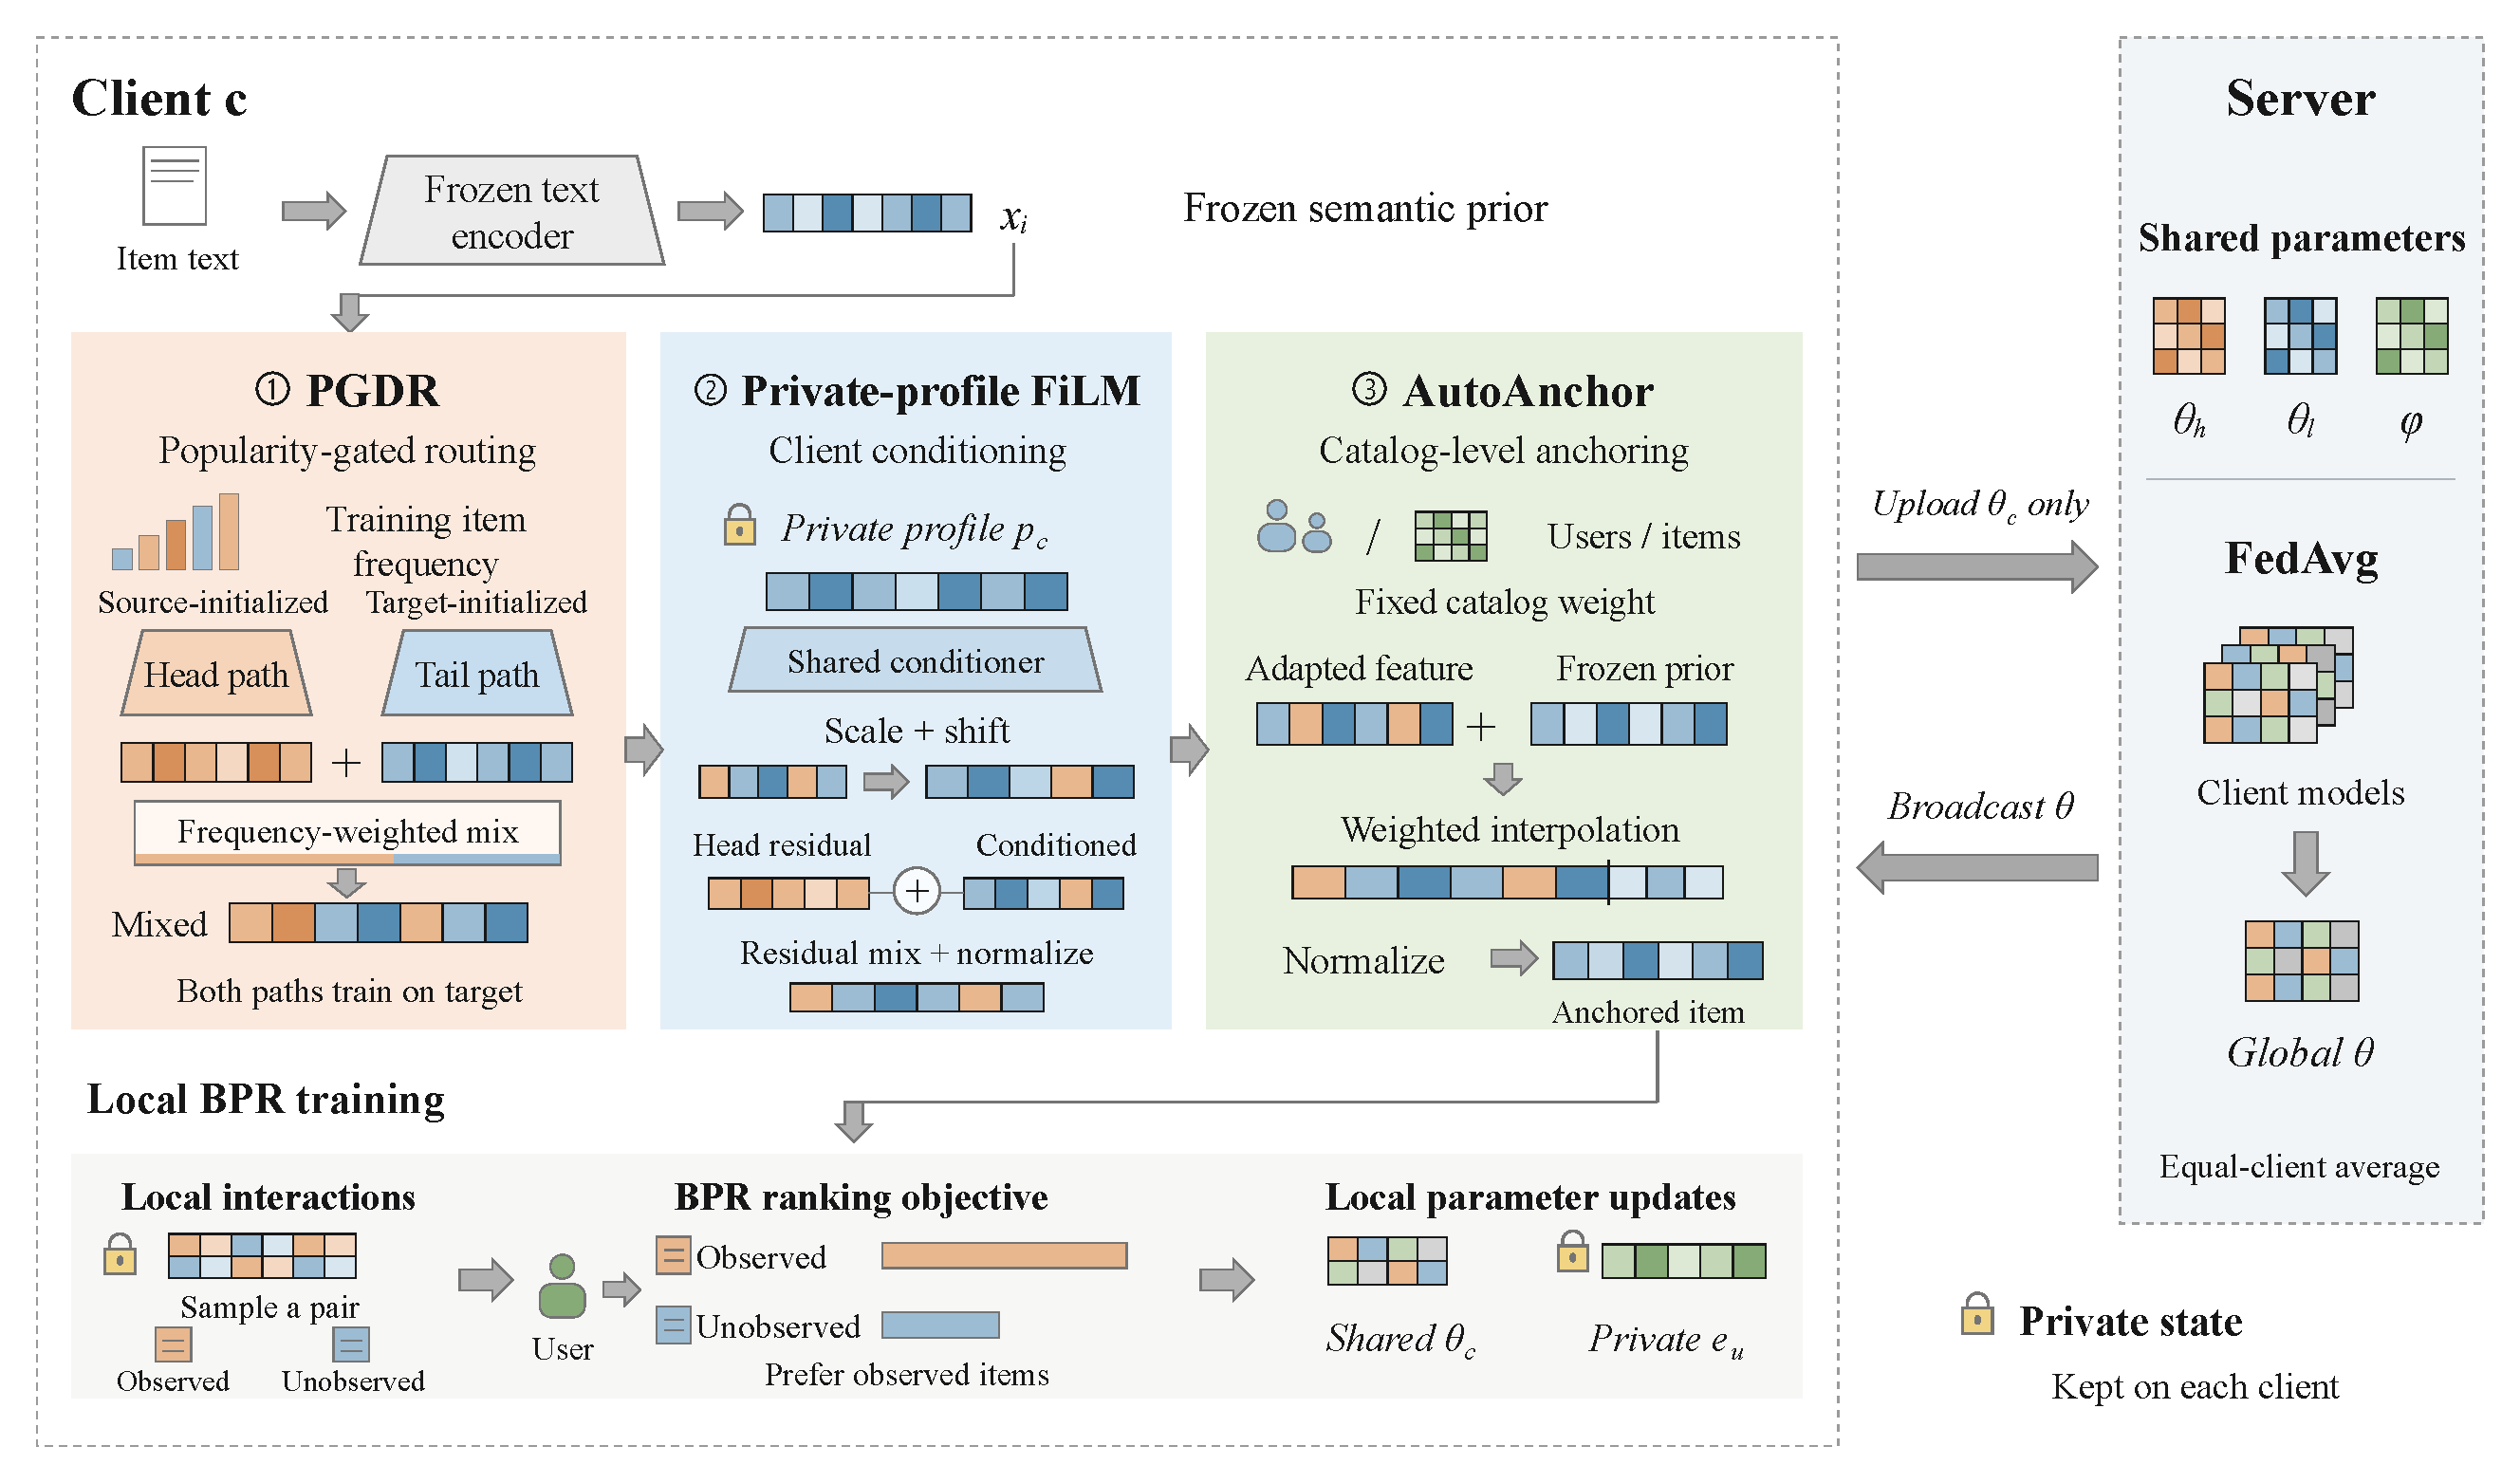
\includegraphics[width=\textwidth]{figures/FedPASA_framework_graphic.pdf}
\caption{FedPASA framework. PGDR combines source-initialized and target-initialized residual adapters according to item frequency. Private-profile FiLM conditions the resulting representations on local interaction semantics, while AutoAnchor integrates the frozen semantic prior. Clients optimize shared model parameters and private user embeddings using BPR, and the server aggregates the shared parameters through FedAvg.}
\label{fig:framework}
\end{figure*}

\subsection{Popularity-Gated Dual-path Routing}
\label{sec:pgdr}

Target items exhibit substantially different interaction frequencies, resulting in different amounts of supervision for semantic adaptation. PGDR explicitly uses item frequency to determine the relative contributions of two residual adaptation paths, enabling frequency-dependent representation learning within a shared model.

Let $\mathrm{freq}(i)$ denote the number of target-domain training interactions containing item $i$. We first construct an inverse-frequency score $\bar q_i=1/\sqrt{\mathrm{freq}(i)+1}$ and normalize it over the target catalog:
\begin{equation}
q_i=\frac{\bar q_i-\min_j \bar q_j}{\max_j \bar q_j-\min_j \bar q_j+\epsilon}.
\label{eq:coldness}
\end{equation}
A threshold $t$ and exponent $\kappa$ further reshape the routing score:
\[
q_i'=\mathrm{clip}\!\big(\tfrac{q_i-t}{1-t},0,1\big)^{\kappa}.
\]
The resulting score $q_i'$ increases as item frequency decreases and controls the relative contribution of the target-initialized path.

PGDR contains two residual adapters, denoted by $A_h$ and $A_l$. The head adapter $A_h$ is initialized from the source-domain adapter, providing transferred semantic adaptation knowledge. The tail adapter $A_l$ is randomly initialized on the target domain and learns complementary transformations from target interactions. Each adapter contains two sequential residual blocks, $v\leftarrow v+F_\ell(v)$, where $F_\ell$ is a bottleneck multilayer perceptron, followed by $\ell_2$ normalization. Both adapters are optimized during target-domain federated training.

The routed item representation is
\begin{equation}
h_i=(1-q_i')\,A_h(x_i)+q_i'\,A_l(x_i).
\label{eq:routing}
\end{equation}
Frequently observed items place greater weight on the source-initialized head path, whereas lower-frequency items receive a larger contribution from the target-initialized tail path. The mixed representation $h_i$ is subsequently passed to the client-conditioning module.

\subsection{Private-Profile Client Conditioning}
\label{sec:conditioning}

Item frequency characterizes supervision at the item level, while clients may observe substantially different semantic regions of the target catalog. To incorporate this client-side heterogeneity, FedPASA constructs a private semantic profile from each client's local interaction history and uses it to condition the routed representation.

For client $c$, let $\mathcal{I}_c$ denote the multiset of items appearing in its training interactions. Repeated interactions retain their multiplicity in the profile construction. The client profile is defined as
\begin{equation}
p_c=\mathrm{norm}\Big(\tfrac{1}{|\mathcal{I}_c|}\sum_{i\in\mathcal{I}_c} x_i\Big).
\label{eq:profile}
\end{equation}
A shared bottleneck network $g_\phi:\mathbb{R}^d\!\to\!\mathbb{R}^{2d}$ maps the profile into feature-wise FiLM parameters:
\begin{equation}
(\gamma_c,\beta_c)=g_\phi(p_c).
\label{eq:filmparams}
\end{equation}
The routed representation $h_i$ is then modulated as
\begin{equation}
\begin{aligned}
m_{c,i}&=h_i\odot(1+\lambda\,\tanh\gamma_c)+\lambda\beta_c,\\
z_{c,i}&=\mathrm{norm}\big((1-\alpha)A_h(x_i)+\alpha m_{c,i}\big).
\end{aligned}
\label{eq:film}
\end{equation}
The coefficient $\lambda$ controls the strength of client-dependent modulation. The $\tanh$ transformation bounds the multiplicative factor to $[1-\lambda,1+\lambda]$, while the additive term provides learned client-specific feature shifts. The coefficient $\alpha\in[0,1]$ controls the contribution of the conditioned representation relative to the head-path residual.

For the conditioning module, only the shared parameters $\phi$ participate in federated communication. The client profile $p_c$ is computed from local training interactions and remains on the client.

\subsection{Catalog-Level Semantic Anchoring}
\label{sec:anchor}

After frequency-aware routing and client conditioning, FedPASA further integrates the frozen semantic representation into the final ranking representation. AutoAnchor determines the contribution of this semantic prior according to target-catalog coverage.

We characterize target-catalog coverage using the user-to-item ratio
\[
\eta_T=|\mathcal{U}_T|/|\mathcal{I}_T|,
\]
where $|\mathcal{U}_T|$ denotes the number of observed target-domain users and $|\mathcal{I}_T|$ denotes the target catalog size. Given coverage thresholds $\tau_l<\tau_h$ and maximum anchor weight $\rho$, AutoAnchor computes
\begin{equation}
\begin{aligned}
\rho_{\mathrm{eff}}&=\rho\cdot\mathrm{clip}\!\Big(\frac{\tau_h-\eta_T}{\tau_h-\tau_l},0,1\Big),\\
z^{\mathrm{anchor}}_{c,i}&=\mathrm{norm}\big((1-\rho_{\mathrm{eff}})\,z_{c,i}+\rho_{\mathrm{eff}}\,x_i\big).
\end{aligned}
\label{eq:anchor}
\end{equation}
The effective weight $\rho_{\mathrm{eff}}$ controls the contribution of the frozen semantic prior. When $\eta_T\leq\tau_l$, the maximum anchor weight $\rho$ is used. As $\eta_T$ increases between $\tau_l$ and $\tau_h$, the prior contribution decreases linearly. For $\eta_T\geq\tau_h$, the final representation relies directly on the adapted representation. Its weight is determined from target-domain catalog statistics and remains fixed throughout federated training and evaluation.

The default catalog-level gate introduces no additional trainable parameters. We additionally evaluate a per-item learnable alternative,
\[
\rho_i=\rho\,\sigma(a_i),
\]
where $a\in\mathbb{R}^{|\mathcal{I}|}$ contains item-specific logits included in federated aggregation. The corresponding comparison is reported in the anchor analysis (\S\ref{sec:exp-anchor}).

\subsection{Federated Training and Local Personalization}
\label{sec:training}

FedPASA jointly learns shared semantic adaptation parameters across clients while maintaining private user representations locally. The shared trainable parameters are $\theta=\{\theta_h,\theta_l,\phi\}$, where $\theta_h$ and $\theta_l$ denote the parameters of the two residual adapters and $\phi$ denotes the parameters of the client-conditioning network. Each client $c$ additionally maintains a private user-embedding table $E_c=\{e_u:u\in\mathcal{U}_c\}$.

During communication round $r$, the server broadcasts the current shared parameters $\theta^{(r)}$ to all participating clients. Each client initializes its local shared-model copy from $\theta^{(r)}$, retains its private user embeddings from the preceding round, and performs $K$ local optimization steps using the BPR objective. The local optimization updates both the shared parameters $\theta_c$ and private user embeddings $E_c$. After local training, each client uploads only $\theta_c$ to the server. Under the default full-participation setting, the server performs equal-client FedAvg:
\[
\theta^{(r+1)}=\frac{1}{|\mathcal{C}|}\sum_{c\in\mathcal{C}}\theta_c.
\]
The federated adaptation stage optimizes the BPR objective without an additional proximal penalty.

After $R$ communication rounds, the resulting global parameters $\theta^{(R)}$ define the shared FedPASA model. We refer to this model before final local personalization as \emph{FedPASA base}. For final personalization, each client initializes its local model from $\theta^{(R)}$, retains its learned private user embeddings, and optimizes
\[
\mathcal{L}_{\mathrm{pers},c}
=
\mathcal{L}_{\mathrm{BPR},c}
+
\frac{\mu_p}{2}\,\|\theta_c-\theta^{(R)}\|_2^2.
\]
The proximal term encourages local adaptation around the final global solution~\citep{li2020federated,li2021ditto}. During this stage, both $\theta_c$ and $E_c$ are updated, while the proximal penalty is applied only to the shared-model parameters $\theta_c$. Each client performs $K_p$ local personalization steps. The resulting personalized parameters remain local and are not uploaded to the server.

Algorithm~\ref{alg:training} summarizes the complete training procedure. Concrete optimization settings are provided in the experimental setup (\S\ref{sec:exp-setup}).

\begin{algorithm}[t]
\caption{FedPASA training and local personalization}
\label{alg:training}
\footnotesize
\begin{algorithmic}[1]
\Require Frozen item features, training histories, clients $\mathcal{C}$, rounds $R$, local steps $K$, personalization steps $K_p$, proximal coefficient $\mu_p$
\State For cross-domain training, optimize a source-domain residual adapter by source BPR and equal-client FedAvg
\State Initialize $\theta_h$ from the source adapter; randomly initialize $\theta_l$ and $\phi$
\State Compute target routing scores $q_i$ from target training frequencies
\State Compute each client profile $p_c$ from its training interactions
\State Compute and fix the catalog-level anchor weight $\rho_{\mathrm{eff}}$
\State Initialize private user tables $E_c=\{e_u:u\in\mathcal{U}_c\}$ for all clients
\State $\theta^{(0)}\gets\{\theta_h,\theta_l,\phi\}$
\For{$r=0,\ldots,R-1$}
    \State Broadcast $\theta^{(r)}$ to all participating clients
    \ForAll{$c\in\mathcal{C}$ \textbf{in parallel}}
        \State $\theta_c\gets\theta^{(r)}$; retain $E_c$ from the preceding round
        \State Take $K$ local steps on $\mathcal{L}_{\mathrm{BPR}}$, updating $(\theta_c,E_c)$
        \State Keep $E_c$ local and upload $\theta_c$
    \EndFor
    \State $\theta^{(r+1)}\gets |\mathcal{C}|^{-1}\sum_{c\in\mathcal{C}}\theta_c$
\EndFor
\State Preserve $\theta^{(R)}$ as the FedPASA base model
\ForAll{$c\in\mathcal{C}$}
    \State $\theta_c\gets\theta^{(R)}$; retain the final $E_c$
    \State $\ell_c\gets\mathcal{L}_{\mathrm{BPR}}+\frac{\mu_p}{2}\|\theta_c-\theta^{(R)}\|_2^2$
    \State Take $K_p$ local personalization steps, updating $(\theta_c,E_c)$
\EndFor
\State \Return Personalized $(\theta_c,E_c)$ stored on each client
\end{algorithmic}
\end{algorithm}

\paragraph{Initialization and local optimization.}
Source-domain training uses one residual adapter together with source-domain user embeddings. The resulting adapter parameters initialize the target-domain head path. The tail path is randomly initialized. The final linear layer of the conditioning network is zero-initialized so that client modulation starts from the shared representation.

Target item frequencies are computed exclusively from target training interactions. Each client profile is computed from its own training-item multiset, with repeated interactions retained. Routing statistics, client profiles, and the catalog-level anchor weight are fixed throughout federated optimization, personalization, and evaluation.

Private user embeddings persist across communication rounds. AdamW optimizer states are reset at the beginning of each local optimization phase. During local training, users are sampled uniformly within a client and positive items are sampled uniformly from the corresponding user's training history. Negative items are sampled from items outside the user's observed training interactions. Dropout is enabled during model updates and disabled during evaluation.

The communication process exchanges only the shared adaptation and conditioning parameters. Raw interaction histories, client profiles, and private user embeddings remain on their respective clients.

\subsection{Analysis of the Adaptation Controls}
\label{sec:theory}

We analyze the main adaptation mechanisms from three perspectives: the relationship between target-estimation reliability and semantic-prior weighting, the geometry of normalized semantic anchoring, and the interaction between popularity routing and client conditioning.

\subsubsection{Bias--Variance Tradeoff of Prior Weighting}

\begin{proposition}[Bias--variance tradeoff]
\label{thm:anchor}
Let $z^*$ denote an ideal target representation and $x$ a semantic prior. Consider an estimated target representation $\hat z=z^*+\varepsilon$, where $\mathbb{E}\varepsilon=0$ and $\mathbb{E}\|\varepsilon\|_2^2=\sigma^2/r$ with $r,\sigma^2>0$. Here, $r$ characterizes the reliability of the target estimate: larger $r$ corresponds to lower estimation variance. Let $b^2=\|x-z^*\|_2^2$ denote the squared bias of the semantic prior. For the interpolated estimate $\tilde z_\omega=(1-\omega)\hat z+\omega x$, we have
\begin{equation}
\mathbb{E}\|\tilde z_\omega-z^*\|_2^2
=(1-\omega)^2\sigma^2/r+\omega^2b^2,
\qquad
\omega^*=\frac{\sigma^2}{\sigma^2+rb^2}.
\label{eq:biasvar}
\end{equation}
When $b>0$, $\omega^*$ decreases as $r$ increases.
\end{proposition}

The optimal weight increases with estimation noise and decreases with prior bias: when target evidence is limited, more of a useful prior should be retained. AutoAnchor operationalizes this principle at the catalog level by using target-catalog coverage to determine the contribution of the frozen semantic prior.

\subsubsection{Geometry of Normalized Semantic Anchoring}

\begin{proposition}[Normalized anchor geometry]
\label{thm:drift}
For fixed unit vectors $x$ and $z$, define $w_\omega=(1-\omega)z+\omega x$, $y_\omega=w_\omega/\|w_\omega\|_2$, and $a=x^\top z$. For $0\le\omega<1/2$,
\begin{equation}
\|w_\omega\|_2\ge1-2\omega>0,
\qquad
\frac{d(x^\top y_\omega)}{d\omega}
=\frac{(1-\omega)(1-a^2)}{\|w_\omega\|_2^3}\ge0.
\label{eq:drift}
\end{equation}
Therefore, $1-x^\top y_\omega$ is non-increasing with respect to the anchor weight $\omega$.
\end{proposition}

This proposition characterizes the geometric effect of normalized semantic interpolation: for a fixed adapted representation, increasing the anchor weight moves the final representation toward the frozen semantic prior. The experimental analysis (\S\ref{sec:exp-drift}) further examines the representation geometry produced after federated optimization.

\subsubsection{Client Conditioning}

The multiplicative part of the FiLM transformation in Eq.~\eqref{eq:film} is $1+\lambda\tanh\gamma_c$. Since $\tanh\gamma_c\in[-1,1]$, the resulting feature-wise multiplicative factors satisfy $1-\lambda\le1+\lambda\tanh\gamma_c\le1+\lambda$. Thus, $\lambda$ directly controls the range of client-dependent multiplicative modulation, while the learned additive term $\lambda\beta_c$ shifts the routed representation according to the client's semantic profile.

\subsubsection{Interaction of Routing and Client Conditioning}

PGDR and client conditioning act on the same semantic representation but control different aspects of adaptation. To make the interaction explicit, consider the case in which FiLM modulation is disabled, i.e., $\lambda=0$. Combining Eqs.~\eqref{eq:routing} and~\eqref{eq:film} gives
\begin{equation}
z_{c,i}=\mathrm{norm}\big((1-\alpha q_i')A_h(x_i)+\alpha q_i'A_l(x_i)\big).
\label{eq:effective-routing}
\end{equation}
The effective coefficient of the target-initialized path is therefore $\alpha q_i'$. The item-frequency-derived score $q_i'$ determines how the two adaptation paths are allocated to each item, while $\alpha$ controls the overall strength of this allocation. Even for the largest routing score $q_i'=1$, the head path retains a contribution of $1-\alpha$.

When FiLM is enabled, client-dependent feature scales and shifts are applied to the frequency-routed representation before normalization and semantic anchoring. Consequently, item frequency controls path combination, whereas the private client profile controls feature-level adjustment.



% !TeX root = ../main.tex
\definecolor{FedPASARow}{RGB}{224,224,250}
\section{Experiments}
\label{sec:exp}
We evaluate FedPASA through four research questions:
\begin{itemize}
\setlength{\itemsep}{0pt}
\setlength{\parskip}{0pt}
\item \textbf{RQ1:} How does FedPASA compare with federated recommendation and semantic-transfer baselines?
\item \textbf{RQ2:} How much does each component contribute beyond additional adapter capacity?
\item \textbf{RQ3:} How do item frequency, client exposure, and catalog coverage explain the gains?
\item \textbf{RQ4:} Does FedPASA remain effective under client heterogeneity, restricted computation, and alternative encoders?
\end{itemize}

\subsection{Datasets}
We evaluate cross-domain recommendation on three Amazon datasets. The benchmark contains all six ordered transfers among Amazon Music (CDs \& Vinyl), Books, and Movies (Movies \& TV)~\citep{ni2019justifying}; their item catalogs are disjoint and no linked users are required. Table~\ref{tab:datasets-main} summarizes the retained data. Users with fewer than three interactions are removed; the last interaction is used for testing, the preceding interaction for validation, and all earlier interactions for training. Appendix~\ref{app:data} gives the evaluation-user counts and preprocessing details.

\begin{table}[t]
\centering\footnotesize
\caption{Dataset statistics after the three-interaction filter. $N$ includes training, validation, and test interactions.}
\label{tab:datasets-main}
\setlength{\tabcolsep}{3.2pt}
\renewcommand{\arraystretch}{1.05}
\begin{tabular}{@{}lrrr@{}}
\toprule
Dataset & Users & Items & $N$ \\
\midrule
Music & 12,315 & 10,680 & 339,923 \\
Books & 262,698 & 170,389 & 10,848,388 \\
Movies & 28,226 & 19,252 & 1,056,608 \\
\bottomrule
\end{tabular}
\end{table}

\begin{table*}[t]
\centering\small
\caption{Sampled-ranking comparison on the first three transfers. FedPASA includes final local personalization. Bold and underline mark the best and second-best results; run counts are given in Appendix~\ref{app:full}.}
\label{tab:cross_main}
\label{tab:native-reproductions}
\setlength{\tabcolsep}{4pt}
\renewcommand{\arraystretch}{1.03}
\begin{tabularx}{\textwidth}{@{}l*{6}{>{\centering\arraybackslash}X}@{}}
\toprule
\textbf{Transfer} & \multicolumn{2}{c}{\textbf{Music$\to$Books}} & \multicolumn{2}{c}{\textbf{Music$\to$Movies}} & \multicolumn{2}{c}{\textbf{Books$\to$Movies}} \\
\cmidrule(lr){2-3} \cmidrule(lr){4-5} \cmidrule(lr){6-7}
\textbf{Method} & HR@20 & NDCG@20 & HR@20 & NDCG@20 & HR@20 & NDCG@20 \\
\midrule
FeDecider~\citep{he2026fedecider} & 0.2011 & 0.0714 & \underline{0.4278} & \underline{0.1823} & \underline{0.3981} & \underline{0.1705} \\
FFMSR~\citep{lu2025ffmsr} & 0.0273 & 0.0116 & 0.1354 & 0.0824 & 0.1231 & 0.0720 \\
FedDCSR~\citep{zhang2024feddcsr} & 0.0254 & 0.0218 & 0.0924 & 0.0724 & 0.0924 & 0.0724 \\
FedMF~\citep{ammad2019federated} & 0.2005 & 0.0715 & 0.2127 & 0.0792 & 0.2127 & 0.0792 \\
FedAvg~\citep{mcmahan2017communication} & 0.1949 & 0.0672 & 0.3440 & 0.1388 & 0.3440 & 0.1388 \\
FedProx~\citep{li2020federated} & 0.1998 & 0.0705 & 0.3381 & 0.1351 & 0.3381 & 0.1351 \\
FedAdam~\citep{reddi2021adaptive} & 0.1986 & 0.0690 & 0.3398 & 0.1359 & 0.3398 & 0.1359 \\
TransFR~\citep{zhang2026transfr} & \underline{0.2058} & \underline{0.0723} & 0.3292 & 0.1283 & 0.3330 & 0.1307 \\
L2-SP~\citep{li2018explicit} & 0.2032 & 0.0718 & 0.3244 & 0.1244 & 0.3141 & 0.1229 \\
FedPer~\citep{arivazhagan2019federated} & 0.2031 & 0.0714 & 0.3410 & 0.1353 & 0.3492 & 0.1397 \\
pFedMe~\citep{dinh2020personalized} & 0.2047 & 0.0719 & 0.3284 & 0.1285 & 0.3368 & 0.1332 \\
FedMoE~\citep{mei2024fedmoe} & 0.2039 & 0.0707 & 0.3424 & 0.1355 & 0.3566 & 0.1444 \\
\rowcolor{FedPASARow}
\textbf{FedPASA} & \textbf{0.2719} & \textbf{0.1159} & \textbf{0.4980} & \textbf{0.2254} & \textbf{0.4948} & \textbf{0.2284} \\
\bottomrule
\end{tabularx}

\end{table*}

\begin{table*}[t]
\centering\small
\caption{Sampled-ranking comparison on the remaining transfers and the six-transfer mean. Metrics and formatting follow Table~\ref{tab:cross_main}.}
\label{tab:cross_main_remaining}
\setlength{\tabcolsep}{4pt}
\renewcommand{\arraystretch}{1.03}
\begin{tabularx}{\textwidth}{@{}l*{8}{>{\centering\arraybackslash}X}@{}}
\toprule
\textbf{Transfer} & \multicolumn{2}{c}{\textbf{Books$\to$Music}} & \multicolumn{2}{c}{\textbf{Movies$\to$Books}} & \multicolumn{2}{c}{\textbf{Movies$\to$Music}} & \multicolumn{2}{c}{\textbf{Six-transfer mean}} \\
\cmidrule(lr){2-3} \cmidrule(lr){4-5} \cmidrule(lr){6-7} \cmidrule(lr){8-9}
\textbf{Method} & HR@20 & NDCG@20 & HR@20 & NDCG@20 & HR@20 & NDCG@20 & HR@20 & NDCG@20 \\
\midrule
FeDecider~\citep{he2026fedecider} & \underline{0.5355} & \underline{0.2283} & 0.2058 & \underline{0.0734} & \underline{0.5380} & \underline{0.2284} & \underline{0.3844} & \underline{0.1590} \\
FFMSR~\citep{lu2025ffmsr} & 0.1585 & 0.0841 & 0.0214 & 0.0094 & 0.1701 & 0.0992 & 0.1060 & 0.0598 \\
FedDCSR~\citep{zhang2024feddcsr} & 0.1090 & 0.0832 & 0.0254 & 0.0218 & 0.1090 & 0.0832 & 0.0756 & 0.0591 \\
FedMF~\citep{ammad2019federated} & 0.2212 & 0.0826 & 0.2005 & 0.0715 & 0.2212 & 0.0826 & 0.2115 & 0.0778 \\
FedAvg~\citep{mcmahan2017communication} & 0.5074 & 0.2129 & 0.1949 & 0.0672 & 0.5074 & 0.2129 & 0.3488 & 0.1396 \\
FedProx~\citep{li2020federated} & 0.5024 & 0.2093 & 0.1998 & 0.0705 & 0.5024 & 0.2093 & 0.3468 & 0.1383 \\
FedAdam~\citep{reddi2021adaptive} & 0.5073 & 0.2098 & 0.1986 & 0.0690 & 0.5073 & 0.2098 & 0.3485 & 0.1382 \\
TransFR~\citep{zhang2026transfr} & 0.5046 & 0.2121 & 0.2001 & 0.0705 & 0.5048 & 0.2115 & 0.3462 & 0.1376 \\
L2-SP~\citep{li2018explicit} & 0.4996 & 0.2083 & 0.2017 & 0.0710 & 0.5040 & 0.2122 & 0.3412 & 0.1351 \\
FedPer~\citep{arivazhagan2019federated} & 0.5052 & 0.2150 & 0.2040 & 0.0721 & 0.5027 & 0.2099 & 0.3509 & 0.1406 \\
pFedMe~\citep{dinh2020personalized} & 0.5054 & 0.2131 & 0.2026 & 0.0712 & 0.5064 & 0.2117 & 0.3474 & 0.1383 \\
FedMoE~\citep{mei2024fedmoe} & 0.5088 & 0.2143 & \underline{0.2064} & 0.0731 & 0.5107 & 0.2141 & 0.3548 & 0.1420 \\
\rowcolor{FedPASARow}
\textbf{FedPASA} & \textbf{0.5408} & \textbf{0.2403} & \textbf{0.2824} & \textbf{0.1249} & \textbf{0.5462} & \textbf{0.2439} & \textbf{0.4390} & \textbf{0.1965} \\
\bottomrule
\end{tabularx}
\end{table*}

\begin{figure*}[t]
\centering
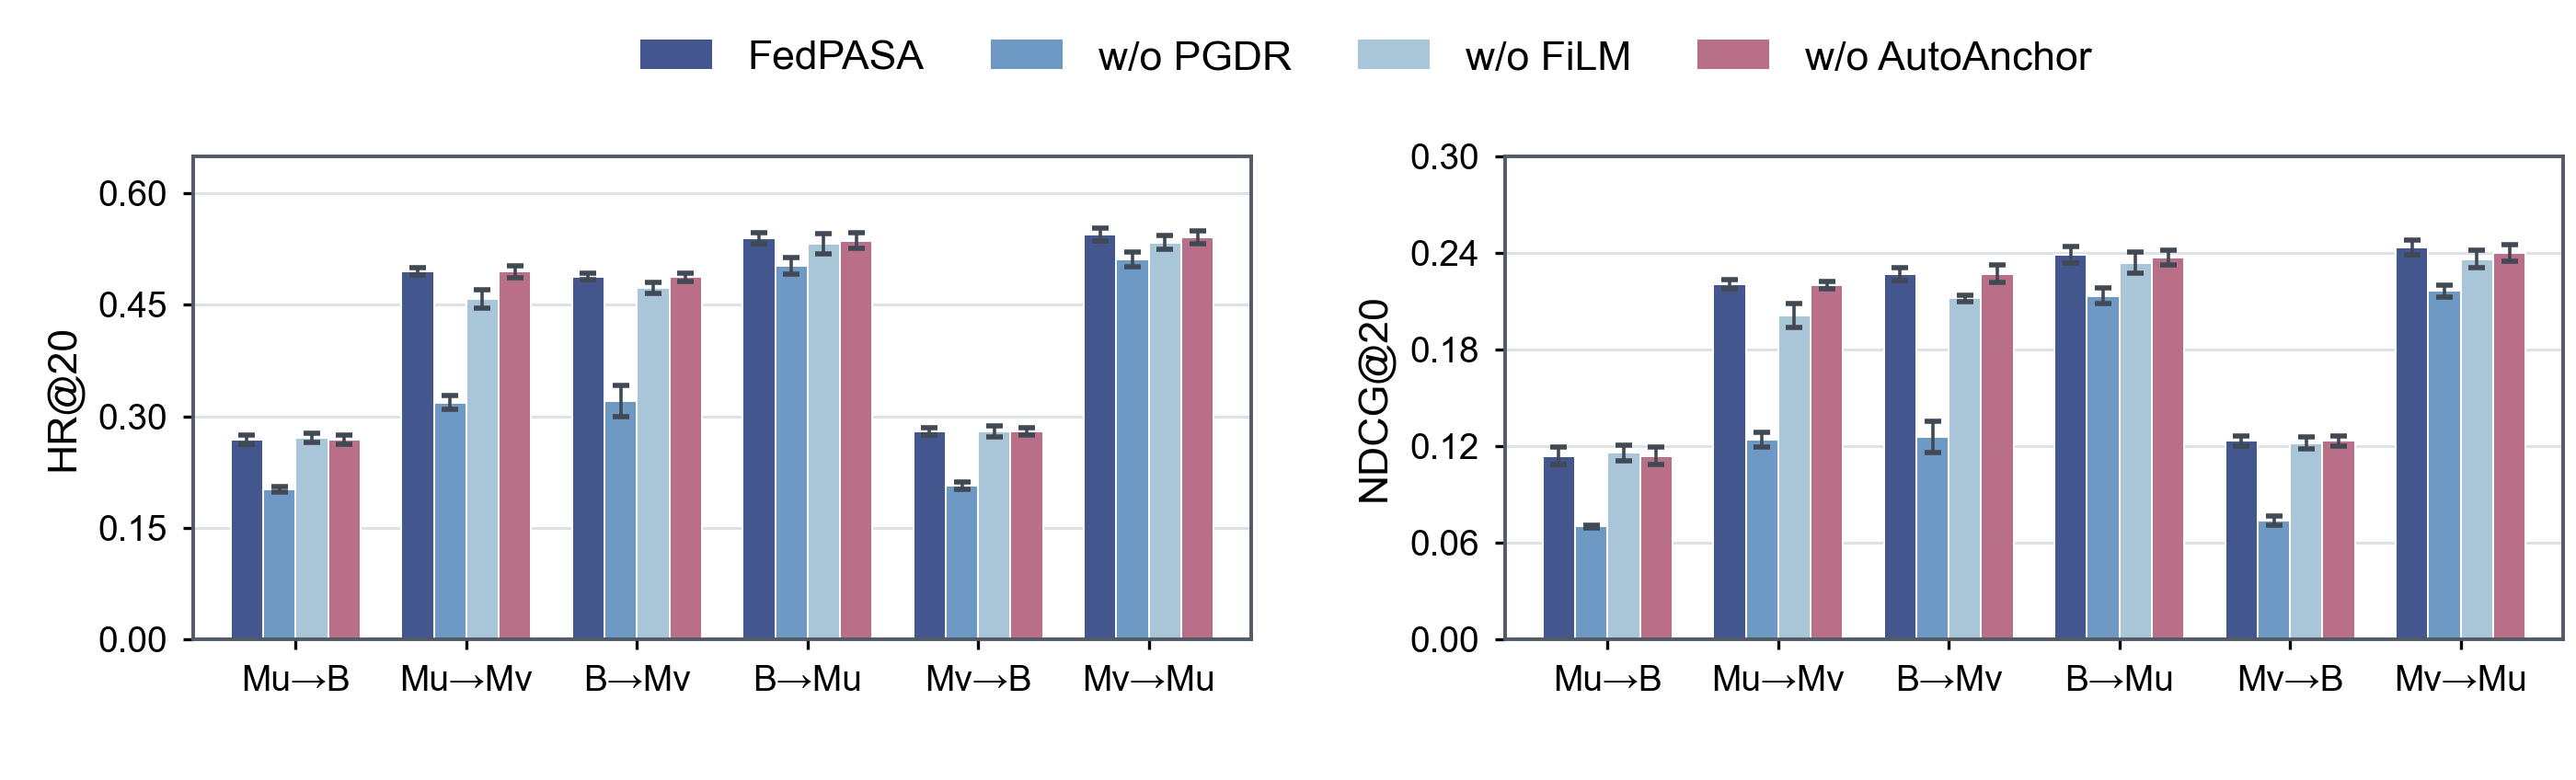
\includegraphics[width=\textwidth]{figures/component_ablation_selected.png}
\caption{Component ablations under 99-negative ranking before personalization (five-seed means $\pm$ SD). Mu: Music; B: Books; Mv: Movies. PGDR contributes most; FiLM and AutoAnchor have target-dependent effects.}
\Description{Two grouped bar charts report HR at 20 and NDCG at 20 for FedPASA and variants without routing, client conditioning, or anchoring across six transfer directions.}
\label{fig:component-ablation}
\end{figure*}

\begin{figure}[t]
\centering
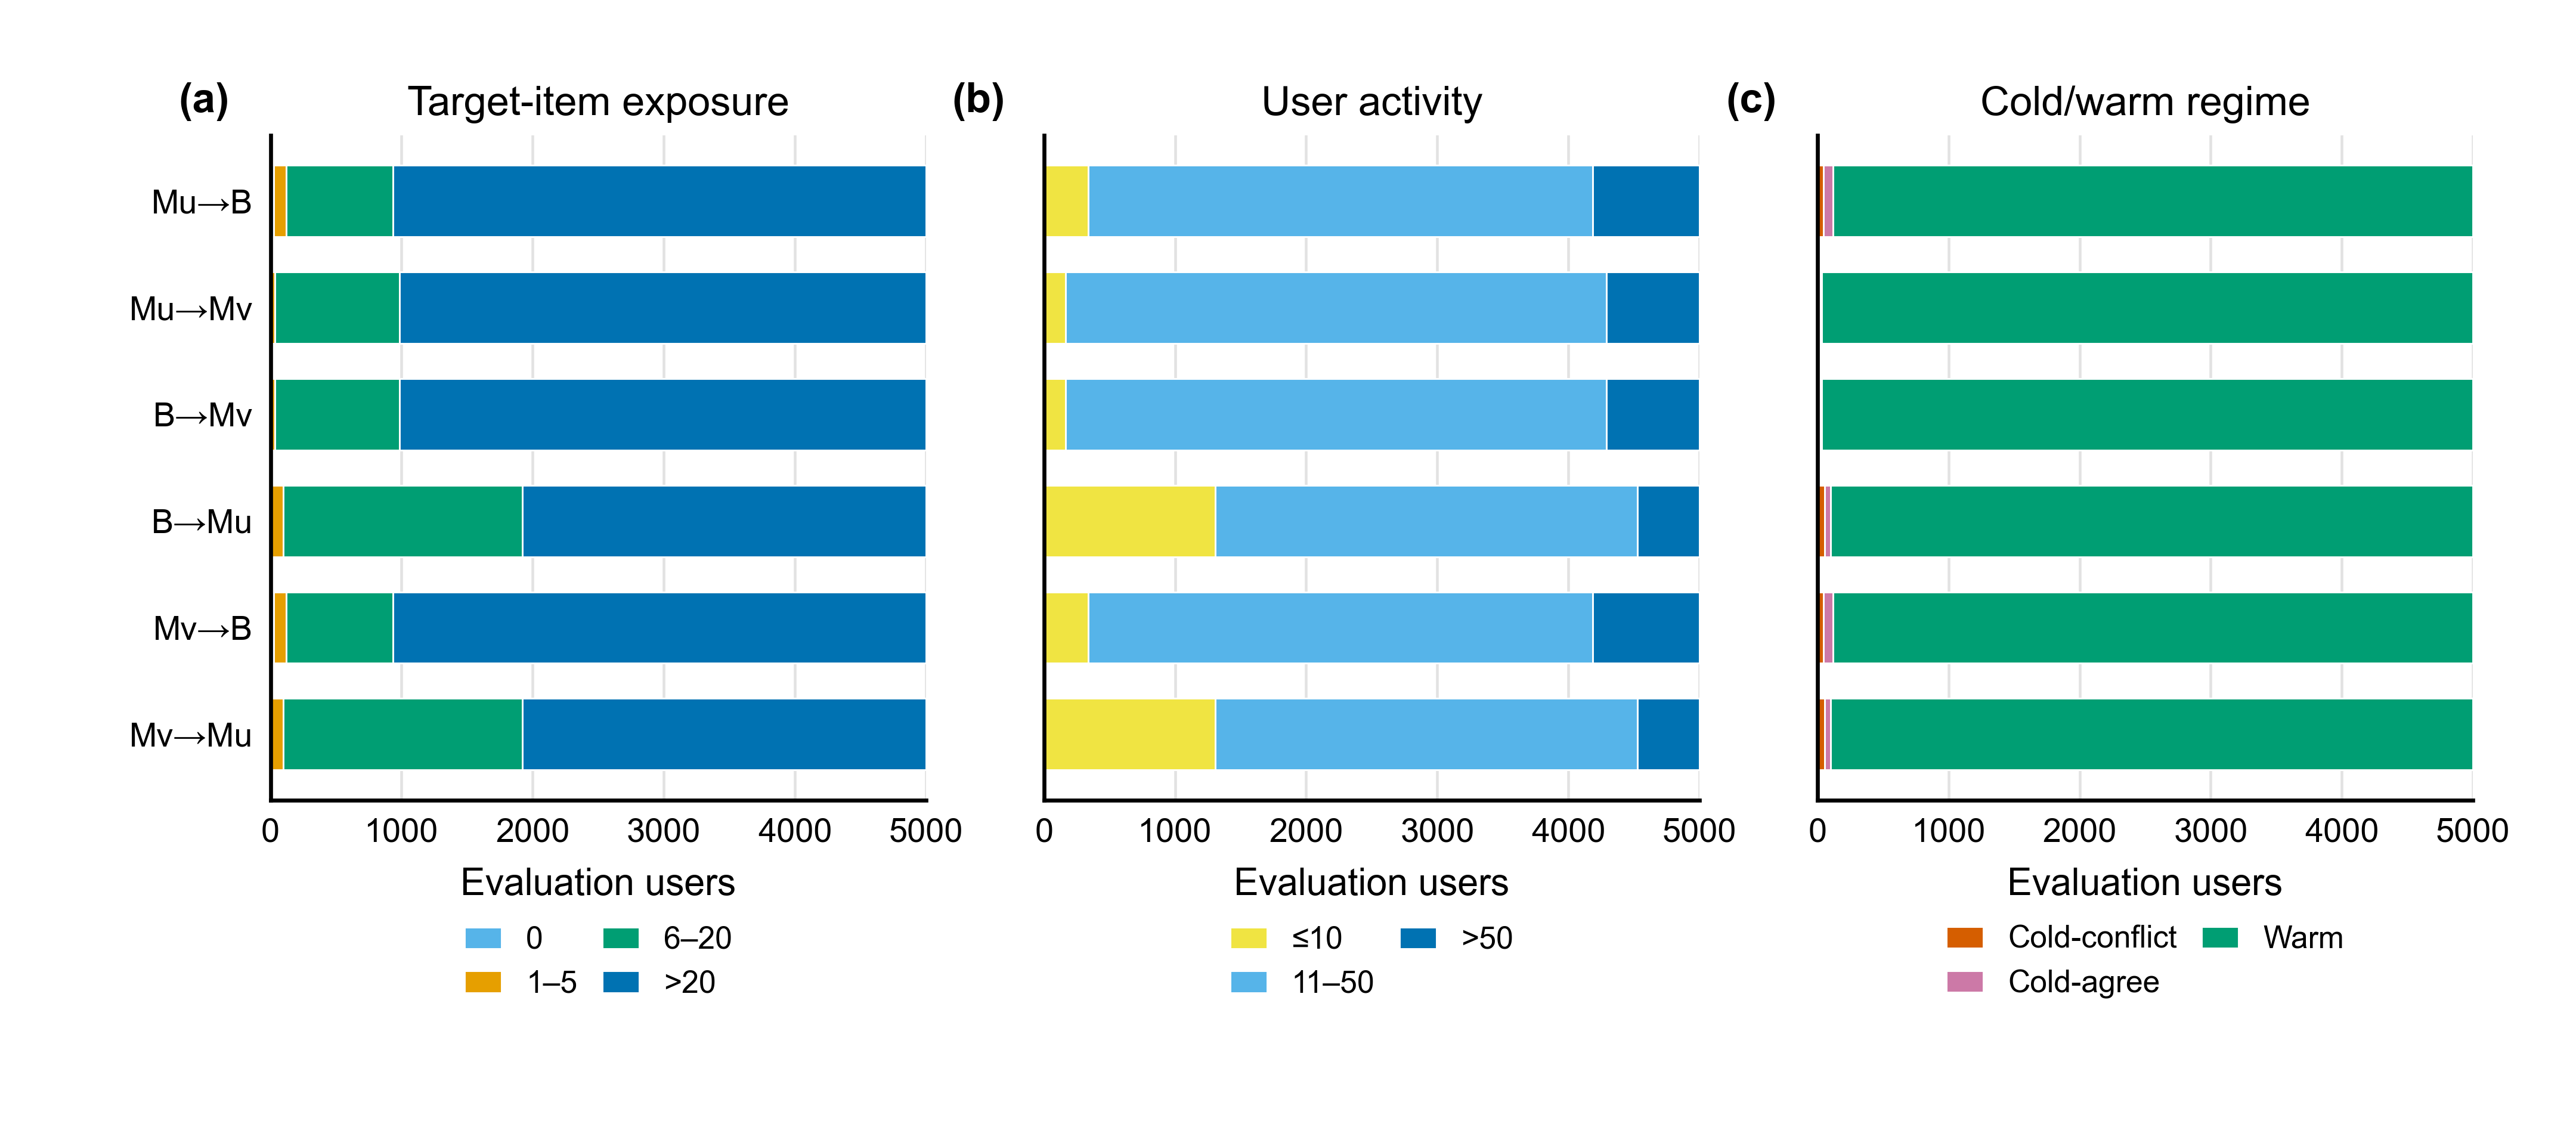
\includegraphics[width=\columnwidth]{figures/evaluation_slice_composition.png}
\caption{Evaluation-user composition: (a) target-item frequency, (b) user activity, and (c) cold/warm groups. Each transfer has 5,000 users. Mu/B/Mv: Music/Books/Movies.}
\Description{Three stacked bar charts show that evaluation users predominantly interact with frequent items, have moderate training activity, and belong to the warm group. The proportions vary across target catalogs.}
\label{fig:evaluation-slice-composition}
\end{figure}

\begin{table*}[t]
\centering\small
\caption{Joint frequency--exposure ablation before local personalization under full-catalog ranking. C/U: low-frequency items locally seen/unseen; W: frequency $>5$.}
\label{tab:joint}\label{tab:joint-ndcg}
\setlength{\tabcolsep}{6pt}
\renewcommand{\arraystretch}{1.12}
\begin{tabular*}{\textwidth}{@{\extracolsep{\fill}}l|rr|rr|rr@{}}
\toprule
\textbf{Model} & \multicolumn{2}{c|}{\textbf{C: low-frequency / seen}} & \multicolumn{2}{c|}{\textbf{U: low-frequency / unseen}} & \multicolumn{2}{c}{\textbf{W: frequency $>5$}} \\
 & HR@20 & NDCG@20 & HR@20 & NDCG@20 & HR@20 & NDCG@20 \\
\midrule
\textbf{FedPASA base} & \textbf{0.0160} & \textbf{0.0070} & \textbf{0.0347} & \textbf{0.0151} & \textbf{0.0102} & \textbf{0.0037} \\
% Lowest nonzero retained observations from outputs/www_v1/cross; pooled across six directions within each seed.
\textbf{w/o PGDR} & 0.0041 & 0.0010 & 0.0039 & 0.0013 & 0.0023 & 0.0007 \\
\textbf{w/o FiLM} & 0.0041 & 0.0018 & 0.0276 & 0.0123 & 0.0037 & 0.0014 \\
\textbf{w/o AutoAnchor} & 0.0082 & 0.0023 & 0.0144 & 0.0047 & 0.0039 & 0.0014 \\
\bottomrule
\end{tabular*}
\end{table*}



\begin{figure*}[t]
\centering
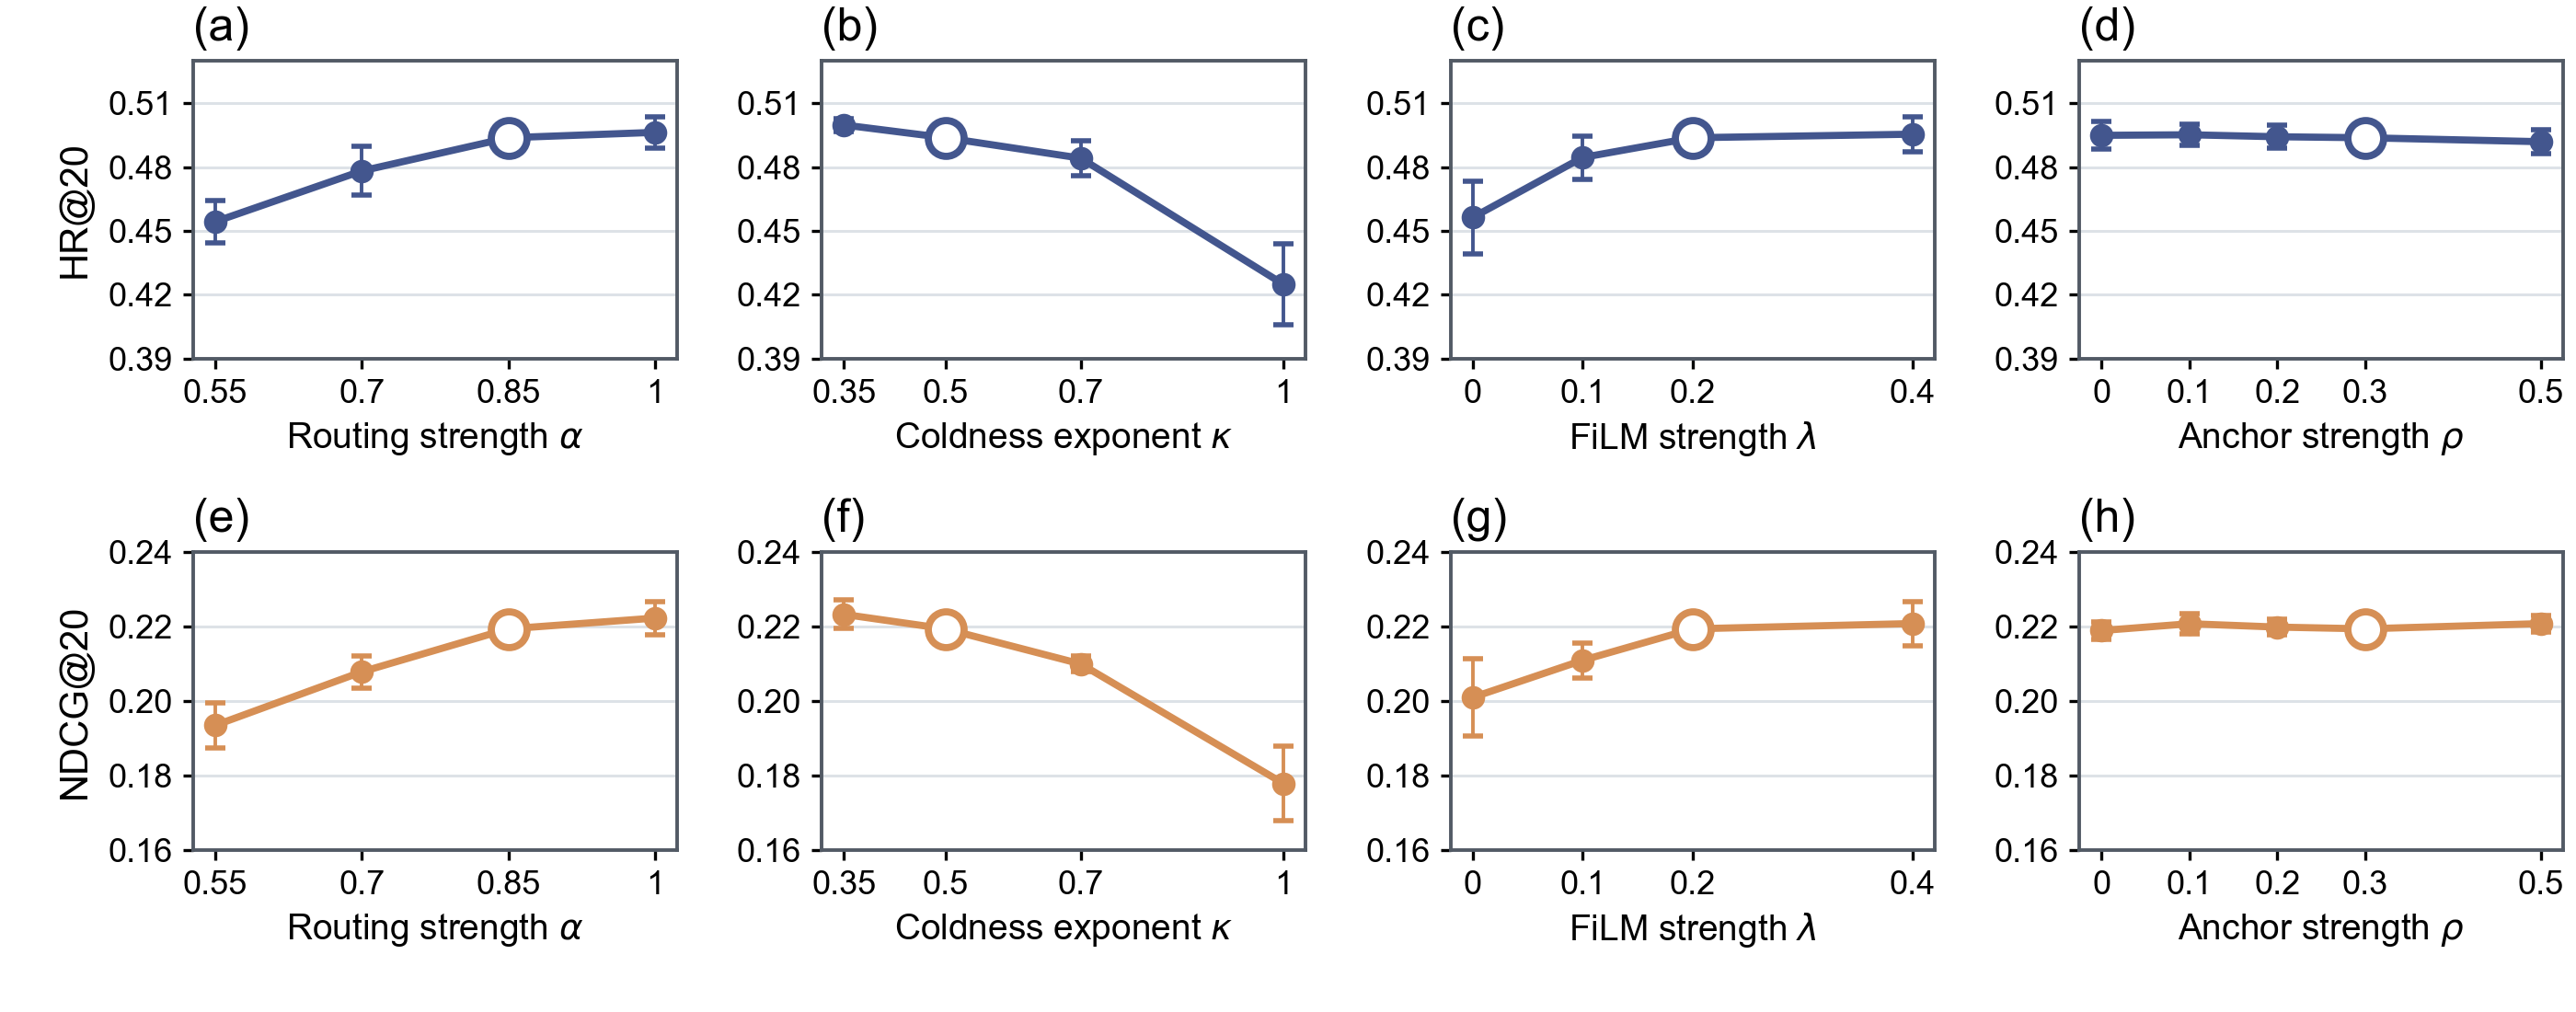
\includegraphics[width=\textwidth]{figures/sensitivity_selected.png}
\caption{Parameter sensitivity on Music$\to$Movies before personalization (99 negatives; three-seed means $\pm$ SD). Top: HR@20; bottom: NDCG@20. Each sweep varies one parameter. Open circles mark validation-selected defaults; vertical scales are shared within each row.}
\Description{Eight panels show the effects of routing strength, coldness exponent, FiLM strength, and anchor strength on HR and NDCG. Routing and coldness have larger effects than anchor strength.}
\label{fig:sensitivity}
\end{figure*}

\subsection{Experimental Settings}
\label{sec:exp-setup}
\subsubsection{Implementation Details}
We encode items with frozen DistilBERT-base-uncased representations ($d=768$) and use two-block residual adapters with bottleneck dimension 64 and dropout 0.1. All adapter methods are optimized with AdamW using a learning rate of $10^{-3}$ and weight decay of $10^{-4}$. Each BPR batch contains 32 positives and three negatives per positive. Cross-domain experiments use five clients and train for $12\times60$ rounds/local steps on Music and Movies and $8\times30$ on Books. FedMF uses 64-dimensional factors and $25\times80$ rounds/local steps. FedPASA sets $\mu=0$ during federation and performs $K_p=40$ personalization steps with $\mu_p=.15$. Validation on Music$\to$Movies selects $(\alpha,\kappa)=(.85,.5)$ and $(\lambda,\rho)=(.2,.3)$, which are fixed for all targets. We report HR and NDCG. Cross-domain evaluation uses a fixed 5,000-user subset with both 99-negative and full-catalog ranking; training and validation items are excluded from candidate sets. Common-backbone results are averaged over five runs. Additional baseline settings are given in Appendix~\ref{app:full}.

\subsubsection{Baselines}
We compare FedPASA with representative recent and classical federated recommendation baselines. \textbf{FeDecider}~\citep{he2026fedecider} uses LLM representations and client-specific directional weights to personalize LoRA aggregation. \textbf{TransFR}~\citep{zhang2026transfr} transfers a source-initialized language-model adapter and performs local personalization. \textbf{FFMSR}~\citep{lu2025ffmsr} transfers text-derived semantic representations in federated recommendation. \textbf{FedDCSR}~\citep{zhang2024feddcsr} disentangles shared and domain-specific factors for federated sequential recommendation. \textbf{FedMoE}~\citep{mei2024fedmoe} personalizes expert subsets through submodel search and modular aggregation. \textbf{FedAdam}~\citep{reddi2021adaptive} applies adaptive server-side optimization, while \textbf{FedProx}~\citep{li2020federated} adds a proximal term to constrain heterogeneous local updates. \textbf{pFedMe}~\citep{dinh2020personalized} couples personalized client parameters to a shared model through a proximal objective. \textbf{FedPer}~\citep{arivazhagan2019federated} combines a globally shared representation with client-specific personalization layers. \textbf{L2-SP}~\citep{li2018explicit} regularizes target parameters toward their source initialization. \textbf{FedAvg} learns one shared target adapter by averaging client updates, and \textbf{FedMF} keeps user factors local while aggregating item factors on the server. In the common-backbone comparison, all methods use the same frozen DistilBERT item features~\citep{sanh2019distilbert}, user partitions, and data splits; other baselines are evaluated with their corresponding datasets and ranking cutoffs.

\subsection{Main Results and Discussion (RQ1)}
\label{sec:exp-main}








\noindent\textit{Evidence-dependent adaptation improves transfer across disjoint catalogs.}
FedPASA leads both sampled-ranking metrics on all six transfers (Tables~\ref{tab:cross_main} and~\ref{tab:cross_main_remaining}), with a mean HR improvement of 14.2\% over FeDecider. The margins vary by target: gains are larger for Books and Movies, whereas the baselines are already competitive on Music. Frozen text features provide a shared semantic space, but do not determine how uneven target supervision should update that space. Frequency-dependent paths offer a plausible explanation for the additional gains; the ablations below isolate the contribution of each component.

\noindent\textit{The advantage extends beyond sampled candidates.}
FedPASA also leads the full-catalog comparison (Table~\ref{tab:full-directions}). The lower absolute accuracy is expected when many more items compete for the same top-ranked positions. Retaining the advantage supports improved discrimination beyond the sampled negatives, although Books remains difficult. This motivates examining both component effects and the item groups contributing to aggregate accuracy.

\subsection{Ablation Study (RQ2)}
\label{sec:exp-ablation}





Figure~\ref{fig:component-ablation} compares FedPASA with variants that remove one component at a time. All variants are evaluated before local personalization to isolate the adaptation modules; Tables~\ref{tab:cross_main} and~\ref{tab:cross_main_remaining} report the final personalized model. Error bars show variation across five seeds.

\noindent\textbf{(1) w/o PGDR.}
Using $h_i=A_h(x_i)$ removes frequency-dependent routing; both metrics decrease on every transfer. The equal-capacity controls retain both paths and the parameter count: constant routing removes item dependence, while shuffling breaks the frequency--weight correspondence. PGDR outperforms both controls, supporting frequency-dependent allocation of adaptation capacity (Table~\ref{tab:ablation}).

\noindent\textbf{(2) w/o FiLM.}
Setting $\lambda=0$ yields $m_{c,i}=h_i$ and removes client-dependent modulation. Average accuracy decreases, with clearer gains on Movies and Music and near-tied results on Books. Client conditioning thus complements routing, with a target-dependent contribution.

\noindent\textbf{(3) w/o AutoAnchor.}
Setting $\rho_{\mathrm{eff}}=0$ removes the frozen-prior contribution in Eq.~\eqref{eq:anchor}. Its average effect is smaller than that of routing or conditioning: Books results are identical because the catalog gate disables anchoring, while Music and Movies show modest changes. Representation drift is examined separately below.

\subsection{Evidence Mechanism Analysis (RQ3)}
\label{sec:exp-buckets}







Table~\ref{tab:joint} compares the component ablations across item groups defined jointly by frequency and local exposure. Each removal lowers both ranking metrics relative to FedPASA base, including for locally seen and locally unseen low-frequency items.

\noindent\textit{Group improvements and aggregate gains are distinct.}
Figure~\ref{fig:evaluation-slice-composition} shows that frequent items and warm cases dominate evaluation, while user activity and exposure vary across target catalogs. Consequently, aggregate metrics weight the groups unequally: strong relative gains in a small low-frequency group need not dominate overall accuracy. The finer slices in Table~\ref{tab:buckets} show that higher-frequency items contribute most of the full-ranking gain over FedAvg. Similar source-free and source-initialized averages (Table~\ref{tab:ablation}) further point to target-side adaptation as the main explanation.

\subsubsection{AutoAnchor and representation drift}
\label{sec:exp-anchor}\label{sec:exp-drift}
Preservation is measured separately from ranking through cosine distance:
\begin{equation}
D=\frac{1}{|\mathcal C||\mathcal I|}\sum_{c\in\mathcal C}\sum_{i\in\mathcal I}
\big(1-\cos(z^{\mathrm{anchor}}_{c,i},x_i)\big).
\end{equation}
Anchoring slightly reduces cold-item distance but increases the all-item average after training (Table~\ref{tab:drift}). Although Eq.~\eqref{eq:anchor} moves a fixed representation toward its prior before normalization, training changes the representation itself. The observed drift and ranking effects therefore depend on the item group and optimization outcome.

\subsection{Generalization and Robustness (RQ4)}
\label{sec:exp-robust}\label{sec:exp-noniid}







\noindent\textit{FedPASA remains effective under heterogeneous conditions.}
FedPASA exceeds TransFR in both metrics under all three non-IID Music$\to$Movies partitions (Table~\ref{tab:external-conditions}). More concentrated activity makes prediction harder, but the advantage persists. The table also examines client counts, fixed computation, partial participation, and update noise.

\noindent\textit{The gains are not tied to one feature encoder.}
The results extend to all evaluated directions with LLaMA features (Table~\ref{tab:external-conditions}), supporting semantic adaptation beyond a particular encoder.

\subsubsection{Sensitivity and statistical analysis}
\label{sec:exp-sens}\label{sec:exp-variability}







Figure~\ref{fig:sensitivity} separates the four adaptation controls. Increasing routing strength $\alpha$ improves both metrics over the tested range, whereas increasing coldness exponent $\kappa$ reduces them. FiLM gains largely saturate near $\lambda=.2$. The flatter response to $\rho$ is consistent with the catalog gate attenuating anchoring on this target. Open circles indicate defaults selected on validation data, not maxima of the plotted test curves. Table~\ref{tab:sensitivity-values} gives the numerical values.

The positive confidence interval for paired HR improvements over the learned-gate baseline supports a repeatable aggregate advantage; Tables~\ref{tab:seed-hr} and~\ref{tab:seed-ndcg} report variability.

% !TeX root = ../main.tex
\section{Conclusion}
FedPASA combines routing by item frequency, client conditioning, and catalog-level anchoring for federated semantic adaptation. Experiments show cross-domain gains with a shared encoder and identify routing as the main contributor at equal model capacity. Conditioning and anchoring have group-dependent effects, motivating more selective adaptation.


\twocolumn
% Reset column height after the final double-column floats.
\makeatletter
\global\@colht\textheight
\global\@colroom\textheight
\global\vsize\textheight
\makeatother
\bibliographystyle{ACM-Reference-Format}
\bibliography{references}


% --- appendix_revised ---
\appendix
% !TeX root = ../main.tex
\section{Dataset Statistics}
\label{app:data}
Table~\ref{tab:datasets} counts users retained after the three-interaction filter. Their last two events form validation and test sets. AutoAnchor uses the retained-user count divided by catalog size. Tests use a fixed subset of 5,000 users in each target domain.

\par\addvspace{6pt}\noindent\begin{minipage}{\columnwidth}\centering\small
\captionof{table}{Retained data after the three-interaction filter. $N$ includes train, validation, and test interactions; ``Eval.'' is the test-user count.}
\label{tab:datasets}
\setlength{\tabcolsep}{2.5pt}
\begin{tabular}{@{}lrrrr@{}}
\toprule
Dataset & Users & Items & $N$ & Eval. \\
\midrule
Music & 12,315 & 10,680 & 339,923 & 5,000 \\
Books & 262,698 & 170,389 & 10,848,388 & 5,000 \\
Movies & 28,226 & 19,252 & 1,056,608 & 5,000 \\
\bottomrule
\end{tabular}
\end{minipage}\par\addvspace{6pt}

Ranking masks training and validation items. The 99-negative sampler and FedMF's unpaired traversal follow \S\ref{sec:exp-setup}. DistilBERT uses normalized masked-mean features (maximum 96 tokens). The encoder check uses LLaMA-2-7B features with a fixed signed block projection to 512 dimensions.

% !TeX root = ../main.tex
\clearpage
\twocolumn[{\section{Full Ranking and Run-to-Run Variation}\label{app:full}

% --- appendix_fullranking_directions ---
\begin{minipage}{\textwidth}
\centering\small
\captionof{table}{Direction-wise full-ranking HR@20 and NDCG@20, complementing Table~\ref{tab:cross_main}. FeDecider is averaged over three runs and the common-backbone methods over five runs. Bold/underline denote the best/second-best values; FedPASA includes final personalization.}
\label{tab:full-directions}
\setlength{\tabcolsep}{3pt}
\renewcommand{\arraystretch}{1.13}
\textbf{(a) HR@20}\par\smallskip
\begin{tabular*}{\linewidth}{@{\extracolsep{\fill}}lrrrrrrr@{}}
\toprule
\textbf{Method} & \textbf{M$\to$B} & \textbf{M$\to$V} & \textbf{B$\to$V} & \textbf{B$\to$M} & \textbf{V$\to$B} & \textbf{V$\to$M} & \textbf{Mean} \\
\midrule
FedMF~\citep{ammad2019federated} & \underline{0.0003} & 0.0022 & 0.0022 & 0.0024 & \underline{0.0003} & 0.0024 & 0.0016 \\
FedAvg~\citep{mcmahan2017communication} & 0.0002 & 0.0037 & 0.0037 & 0.0125 & 0.0002 & 0.0125 & 0.0055 \\
FedProx~\citep{li2020federated} & 0.0001 & 0.0041 & 0.0041 & 0.0130 & 0.0001 & 0.0130 & 0.0057 \\
FedAdam~\citep{reddi2021adaptive} & 0.0001 & 0.0033 & 0.0033 & 0.0110 & 0.0001 & 0.0110 & 0.0048 \\
TransFR~\citep{zhang2026transfr} & 0.0001 & 0.0037 & 0.0030 & 0.0126 & 0.0000 & 0.0132 & 0.0054 \\
L2-SP~\citep{li2018explicit} & 0.0000 & 0.0029 & 0.0028 & 0.0132 & 0.0001 & 0.0132 & 0.0054 \\
FedPer~\citep{arivazhagan2019federated} & 0.0001 & 0.0034 & 0.0040 & 0.0127 & 0.0002 & 0.0119 & 0.0054 \\
pFedMe~\citep{dinh2020personalized} & 0.0001 & 0.0029 & 0.0034 & 0.0125 & 0.0000 & 0.0132 & 0.0053 \\
FedMoE~\citep{mei2024fedmoe} & 0.0001 & 0.0041 & 0.0045 & 0.0134 & 0.0002 & 0.0137 & 0.0060 \\
FeDecider~\citep{he2026fedecider} & 0.0001 & \underline{0.0071} & \underline{0.0055} & \underline{0.0136} & 0.0001 & \underline{0.0145} & \underline{0.0068} \\
\midrule
\textbf{FedPASA} & \textbf{0.0017} & \textbf{0.0126} & \textbf{0.0140} & \textbf{0.0177} & \textbf{0.0018} & \textbf{0.0188} & \textbf{0.0111} \\
\bottomrule
\end{tabular*}
\par\medskip
\textbf{(b) NDCG@20}\par\smallskip
\begin{tabular*}{\linewidth}{@{\extracolsep{\fill}}lrrrrrrr@{}}
\toprule
\textbf{Method} & \textbf{M$\to$B} & \textbf{M$\to$V} & \textbf{B$\to$V} & \textbf{B$\to$M} & \textbf{V$\to$B} & \textbf{V$\to$M} & \textbf{Mean} \\
\midrule
FedMF~\citep{ammad2019federated} & \underline{0.0001} & 0.0009 & 0.0009 & 0.0009 & \underline{0.0001} & 0.0009 & 0.0006 \\
FedAvg~\citep{mcmahan2017communication} & 0.0000 & 0.0015 & 0.0015 & 0.0043 & 0.0000 & 0.0043 & 0.0019 \\
FedProx~\citep{li2020federated} & 0.0000 & 0.0015 & 0.0015 & 0.0047 & 0.0000 & 0.0047 & 0.0021 \\
FedAdam~\citep{reddi2021adaptive} & 0.0000 & 0.0011 & 0.0011 & 0.0041 & 0.0000 & 0.0041 & 0.0018 \\
TransFR~\citep{zhang2026transfr} & 0.0000 & 0.0012 & 0.0011 & 0.0047 & 0.0000 & 0.0050 & 0.0020 \\
L2-SP~\citep{li2018explicit} & 0.0000 & 0.0011 & 0.0011 & 0.0046 & 0.0000 & 0.0049 & 0.0019 \\
FedPer~\citep{arivazhagan2019federated} & 0.0000 & 0.0012 & 0.0014 & 0.0045 & 0.0001 & 0.0042 & 0.0019 \\
pFedMe~\citep{dinh2020personalized} & 0.0000 & 0.0009 & 0.0012 & 0.0046 & 0.0000 & 0.0049 & 0.0019 \\
FedMoE~\citep{mei2024fedmoe} & 0.0000 & 0.0015 & 0.0016 & \underline{0.0050} & 0.0001 & 0.0052 & 0.0022 \\
FeDecider~\citep{he2026fedecider} & 0.0000 & \underline{0.0025} & \underline{0.0019} & 0.0049 & 0.0001 & \underline{0.0055} & \underline{0.0025} \\
\midrule
\textbf{FedPASA} & \textbf{0.0006} & \textbf{0.0046} & \textbf{0.0050} & \textbf{0.0065} & \textbf{0.0009} & \textbf{0.0069} & \textbf{0.0041} \\
\bottomrule
\end{tabular*}
\end{minipage}

\par\medskip

% --- appendix_results_top ---
\par\noindent\begin{minipage}{\textwidth}\centering\footnotesize
\captionof{table}{Sampled HR@20 mean and sample SD. FeDecider uses three runs; other methods use five. Mean-column SD is computed after averaging six directions within each run.}\label{tab:seed-hr}
\setlength{\tabcolsep}{2.5pt}
\begin{tabular*}{\linewidth}{@{\extracolsep{\fill}}lrrrrrrr@{}}
\toprule
Method & M$\to$B & M$\to$V & B$\to$V & B$\to$M & V$\to$B & V$\to$M & Mean \\
\midrule
TransFR~\citep{zhang2026transfr} & 0.2058$\pm$0.0051 & 0.3292$\pm$0.0065 & 0.3330$\pm$0.0210 & 0.5046$\pm$0.0127 & 0.2001$\pm$0.0071 & 0.5048$\pm$0.0074 & 0.3462$\pm$0.0066 \\
FedMoE~\citep{mei2024fedmoe} & 0.2039$\pm$0.0032 & 0.3424$\pm$0.0120 & 0.3566$\pm$0.0077 & 0.5088$\pm$0.0056 & 0.2064$\pm$0.0059 & 0.5107$\pm$0.0085 & 0.3548$\pm$0.0042 \\
FeDecider~\citep{he2026fedecider} & 0.2011$\pm$0.0023 & 0.4278$\pm$0.0055 & 0.3981$\pm$0.0131 & 0.5355$\pm$0.0240 & 0.2058$\pm$0.0029 & 0.5380$\pm$0.0214 & 0.3844$\pm$0.0070 \\
FedPASA base & 0.2692$\pm$0.0063 & 0.4950$\pm$0.0055 & 0.4881$\pm$0.0039 & 0.5394$\pm$0.0072 & 0.2796$\pm$0.0053 & 0.5449$\pm$0.0085 & 0.4360$\pm$0.0044 \\
FedPASA & 0.2719$\pm$0.0068 & 0.4980$\pm$0.0085 & 0.4948$\pm$0.0053 & 0.5408$\pm$0.0126 & 0.2824$\pm$0.0052 & 0.5462$\pm$0.0094 & 0.4390$\pm$0.0058 \\
\bottomrule
\end{tabular*}
\end{minipage}\par\addvspace{6pt}
\par\noindent\begin{minipage}{\textwidth}\centering\footnotesize
\captionof{table}{Sampled NDCG@20 mean and sample SD. FeDecider uses three runs; other methods use five. Mean-column SD is computed after averaging six directions within each run.}\label{tab:seed-ndcg}
\setlength{\tabcolsep}{2.5pt}
\begin{tabular*}{\linewidth}{@{\extracolsep{\fill}}lrrrrrrr@{}}
\toprule
Method & M$\to$B & M$\to$V & B$\to$V & B$\to$M & V$\to$B & V$\to$M & Mean \\
\midrule
TransFR~\citep{zhang2026transfr} & 0.0723$\pm$0.0032 & 0.1283$\pm$0.0028 & 0.1307$\pm$0.0090 & 0.2121$\pm$0.0044 & 0.0705$\pm$0.0030 & 0.2115$\pm$0.0042 & 0.1376$\pm$0.0027 \\
FedMoE~\citep{mei2024fedmoe} & 0.0707$\pm$0.0010 & 0.1355$\pm$0.0035 & 0.1444$\pm$0.0027 & 0.2143$\pm$0.0031 & 0.0731$\pm$0.0024 & 0.2141$\pm$0.0059 & 0.1420$\pm$0.0019 \\
FeDecider~\citep{he2026fedecider} & 0.0714$\pm$0.0014 & 0.1823$\pm$0.0055 & 0.1705$\pm$0.0093 & 0.2283$\pm$0.0099 & 0.0734$\pm$0.0027 & 0.2284$\pm$0.0095 & 0.1590$\pm$0.0042 \\
FedPASA base & 0.1140$\pm$0.0053 & 0.2204$\pm$0.0031 & 0.2268$\pm$0.0042 & 0.2389$\pm$0.0051 & 0.1232$\pm$0.0034 & 0.2432$\pm$0.0046 & 0.1944$\pm$0.0032 \\
FedPASA & 0.1159$\pm$0.0054 & 0.2254$\pm$0.0053 & 0.2284$\pm$0.0032 & 0.2403$\pm$0.0076 & 0.1249$\pm$0.0035 & 0.2439$\pm$0.0069 & 0.1965$\pm$0.0035 \\
\bottomrule
\end{tabular*}
\end{minipage}\par\addvspace{6pt}


\par\noindent\begin{minipage}{\textwidth}\small\textit{Baseline settings.} The FedMoE comparison uses two shared adapters with a learned gate, without client-specific submodel search or modular aggregation. FedDCSR reports target-domain results, so transfers to the same target share a value. FFMSR retains its corresponding evaluation setting.\end{minipage}\par
}]

% !TeX root = ../main.tex
\clearpage
\twocolumn[{\section{Additional Baseline Comparisons and Ablations}\label{app:external}}]

% --- tables_external_baselines ---
\par\noindent\begin{minipage}{\columnwidth}\centering\small
\captionof{table}{Cross-domain recommendation on Amazon Music/Books/Movies~\citep{zhang2026transfr}. Each cell contains HR@10/NDCG@10.}
\label{tab:transfr-published}
\setlength{\tabcolsep}{2.5pt}
\begin{tabular}{@{}lcccc@{}}
\toprule
Method & M$\to$B & M$\to$V & B$\to$V & Mean \\
\midrule
CMF~\citep{singh2008relational} & .1833/.0955 & .1378/.0764 & .1455/.0662 & .1555/.0794 \\
EMCDR~\citep{man2017cross} & .2149/.1121 & .1893/.0901 & .1652/.0705 & .1898/.0909 \\
DisenCDR~\citep{cao2022disencdr} & .2243/.1182 & .1988/.0923 & .1912/.0821 & .2048/.0975 \\
FCF~\citep{ammad2019federated} & .1380/.0663 & .1154/.0583 & .1004/.0421 & .1179/.0556 \\
IFedRec~\citep{zhang2024ifedrec} & .1981/.0834 & .1810/.0673 & .1703/.0497 & .1831/.0668 \\
FELLRec~\citep{zhao2025fellrec} & .2003/.0995 & .1844/.0812 & .1731/.0831 & .1859/.0879 \\
FedCT~\citep{liu2021fedct} & .2034/.1122 & .1765/.0899 & .1585/.0845 & .1795/.0955 \\
FedDCSR~\citep{zhang2024feddcsr} & .2217/.1085 & .1881/.0892 & .1719/.0732 & .1939/.0903 \\
\textbf{TransFR}~\citep{zhang2026transfr} & \textbf{.2335/.1133} & \textbf{.2123/.0934} & \textbf{.2089/.0893} & \textbf{.2182/.0987} \\
\bottomrule
\end{tabular}

\end{minipage}\par\addvspace{8pt}

% --- tables_ablation_revised ---
\par\noindent\begin{minipage}{\columnwidth}\centering\footnotesize
\captionof{table}{Component and capacity controls: six-transfer means over five runs. Only the final row includes personalization.}\label{tab:ablation}
\setlength{\tabcolsep}{1.5pt}
\begin{tabular*}{\linewidth}{@{\extracolsep{\fill}}lrr@{}}
\toprule
Model & HR@20 & NDCG@20 \\
\midrule
FedPASA base & 0.4360 & 0.1944 \\
w/o PGDR & 0.3434 & 0.1373 \\
w/o FiLM & 0.4245 & 0.1867 \\
w/o AutoAnchor & 0.4346 & 0.1934 \\
Constant routing & 0.3481 & 0.1404 \\
Random routing & 0.3381 & 0.1350 \\
Per-item anchor & 0.4365 & 0.1950 \\
Source-free base & 0.4362 & 0.1958 \\
FedMoE~\citep{mei2024fedmoe} & 0.3548 & 0.1420 \\
Personalized & 0.4390 & 0.1965 \\
\bottomrule
\end{tabular*}
\end{minipage}\par\addvspace{6pt}


% --- appendix_notation ---
\subsection{Notation}
\label{app:notation}
\par\addvspace{3pt}\noindent\begin{minipage}{\columnwidth}\centering\footnotesize
\captionof{table}{Notation used in FedPASA.}
\label{tab:notation}
\setlength{\tabcolsep}{3pt}
\begin{tabularx}{\columnwidth}{@{}lX@{}}
\toprule
Symbol & Definition \\
\midrule
$x_i$, $e_u$ & Unit frozen item vector; private user vector \\
$A_h,A_l$ & Source-initialized and target-initialized adapters \\
$F_\ell$ & Bottleneck MLP in residual block $\ell$ \\
$q_i,q_i'$ & Normalized and sharpened inverse-frequency scores \\
$t,\kappa$ & Routing threshold and exponent \\
$h_i,m_{c,i},z_{c,i}$ & Routed, modulated, and normalized residual features \\
$p_c,g_\phi$ & Private client profile; shared FiLM conditioner \\
$\alpha,\lambda$ & Residual-mixture and FiLM strengths \\
$\eta_T,\rho_{\mathrm{eff}}$ & User-to-item ratio; resulting anchor weight \\
$\rho,\tau_l,\tau_h$ & Maximum anchor weight and ratio thresholds \\
$\Theta,\mu,\mu_p$ & Shared parameters; federation and personalization penalties \\
$r,b^2,\sigma^2$ & Reliability, squared prior bias, and noise scale in Proposition~\ref{thm:anchor} \\
\bottomrule
\end{tabularx}
\end{minipage}\par\addvspace{3pt}

\newpage
\par\noindent\begin{minipage}{\columnwidth}\centering\small
\captionof{table}{FFMSR and PFCR recommendation performance. R: recall; N: NDCG.}
\label{tab:ffmsr-pfcr-published}
\textbf{FFMSR}~\citep{lu2025ffmsr}\\[2pt]
\setlength{\tabcolsep}{2.5pt}
\begin{tabular}{@{}lrrrr@{}}
\toprule
Domain & R10 & R50 & N10 & N50 \\
\midrule
Office & .1312 & .2069 & .0890 & .1054 \\
Arts & .1257 & .2377 & .0711 & .0955 \\
OnlineRetail & .1655 & .4110 & .0763 & .1300 \\
Pantry & .0695 & .1818 & .0326 & .0568 \\
\bottomrule
\end{tabular}
\\[4pt]
\textbf{PFCR (full prompting)}~\citep{guo2024pfcr}\\[2pt]
\begin{tabular}{@{}lrrrr@{}}
\toprule
Domain & R10 & R50 & N10 & N50 \\
\midrule
Office & .1206 & .1938 & .0782 & .0941 \\
Arts & .1153 & .2199 & .0677 & .0904 \\
OnlineRetail & .1561 & .3982 & .0739 & .1266 \\
Pantry & .0616 & .1591 & .0293 & .0503 \\
\bottomrule
\end{tabular}

\end{minipage}\par\addvspace{8pt}
\par\noindent\begin{minipage}{\columnwidth}\centering\small
\captionof{table}{FedCRF full-ranking performance across domain pairs~\citep{guo2026fedcrf}.}
\label{tab:external-published-b}
\setlength{\tabcolsep}{2.5pt}
\begin{tabular}{@{}llrrrr@{}}
\toprule
Pair & Domain & R@10 & R@20 & N@10 & N@20 \\
\midrule
Kitchen--Food & Kitchen & .04465 & .06601 & .02523 & .03112 \\
 & Food & .11078 & .16105 & .06708 & .08193 \\
Care--Beauty & Care & .07115 & .09897 & .04250 & .05001 \\
 & Beauty & .09342 & .13384 & .05398 & .06513 \\
Food--OnlineRetail & Food & .11142 & .16185 & .06713 & .08189 \\
 & OnlineRetail & .22864 & .31488 & .19232 & .23368 \\
\bottomrule
\end{tabular}

\end{minipage}\par\addvspace{8pt}

% --- tables_frequency_slices ---

\par\noindent\begin{minipage}{\columnwidth}\centering\footnotesize
\captionof{table}{Fine-grained frequency slices (99-negative ranking; unpersonalized models).}\label{tab:buckets}
\setlength{\tabcolsep}{2.5pt}
\begin{tabular*}{\linewidth}{@{\extracolsep{\fill}}lrrr@{}}
\toprule
Frequency & Method & HR@20 & NDCG@20 \\
\midrule
Unseen & TransFR~\citep{zhang2026transfr} & 0.3020 & 0.1070 \\
 & FedMoE~\citep{mei2024fedmoe} & 0.2460 & 0.0927 \\
 & FedPASA base & 0.5360 & 0.3783 \\
1--5 & TransFR~\citep{zhang2026transfr} & 0.3711 & 0.1562 \\
 & FedMoE~\citep{mei2024fedmoe} & 0.3915 & 0.1662 \\
 & FedPASA base & 0.3439 & 0.2045 \\
6--20 & TransFR~\citep{zhang2026transfr} & 0.3465 & 0.1395 \\
 & FedMoE~\citep{mei2024fedmoe} & 0.3541 & 0.1438 \\
 & FedPASA base & 0.2631 & 0.0990 \\
>20 & TransFR~\citep{zhang2026transfr} & 0.3455 & 0.1361 \\
 & FedMoE~\citep{mei2024fedmoe} & 0.3544 & 0.1404 \\
 & FedPASA base & 0.4956 & 0.2258 \\
\bottomrule
\end{tabular*}
\end{minipage}\par\addvspace{6pt}
\noindent The unseen slice contains 20 nonempty evaluations (mean support: 13 users); other slices contain 30. Evaluations with zero hits are included.\par





% !TeX root = ../main.tex
\clearpage
\twocolumn[{\section{Hyperparameters and Robustness Analysis}\label{app:extra}\label{app:sampled}



% --- appendix_fullranking_top ---
\begin{minipage}{\textwidth}\centering\small
\captionof{table}{Validation-only selection on Music$\to$Movies (mean sampled HR@20 over three runs; eight rounds, 30 local steps). Stage 1 fixes $\lambda=.4,\rho=.2$; Stage 2 fixes the selected $\alpha=.85,\kappa=.5$. The final choice is $(.85,.5,.2,.3)$.}\label{tab:validation-grid}
\begin{minipage}{.48\textwidth}\centering
\begin{tabular}{lrrr}\toprule
$\alpha\backslash\kappa$ & .5 & .7 & 1.0\\\midrule
0.4 & 0.2807 & 0.2640 & 0.2517\\
0.55 & 0.3261 & 0.2871 & 0.2626\\
0.7 & 0.3657 & 0.3139 & 0.2721\\
0.85 & 0.3851 & 0.3541 & 0.2883\\
\bottomrule\end{tabular}\end{minipage}\hfill\begin{minipage}{.48\textwidth}\centering
\begin{tabular}{lrrr}\toprule
$\lambda\backslash\rho$ & .1 & .2 & .3\\\midrule
0.2 & 0.3917 & 0.3917 & 0.3925\\
0.4 & 0.3879 & 0.3851 & 0.3893\\
0.6 & 0.3842 & 0.3874 & 0.3817\\
\bottomrule\end{tabular}\end{minipage}\end{minipage}\par\addvspace{6pt}


}]

% --- appendix_settings_left ---
\subsection{Configuration}
\label{app:hyper}
\par\addvspace{3pt}\noindent\begin{minipage}{\columnwidth}\centering\footnotesize
\captionof{table}{Default configuration. Sensitivity experiments vary one setting at a time.}
\label{tab:hyper}
\setlength{\tabcolsep}{3pt}
\begin{tabularx}{\columnwidth}{@{}p{.36\columnwidth}X@{}}
\toprule
Setting & Value \\
\midrule
Frozen encoder & DistilBERT-base-uncased, $d=768$ \\
Adapter & 2 residual blocks; bottleneck 64; dropout 0.1 \\
Optimizer & AdamW; lr $10^{-3}$; weight decay $10^{-4}$ \\
BPR batches & 32 positives; 3 negatives/positive; logit scale 10 \\
Federation & Cross: $12\times60$ rounds/steps; target Books: $8\times30$ \\
Clients & 5 \\
Mixing / FiLM & $\alpha=.85$, $t=0$, $\kappa=.5$, $\lambda=.2$ \\
Anchor & $\rho=.3$; $[\tau_l,\tau_h]=[1,1.5]$ \\
Proximal terms & FedProx: $.1$; L2-SP: $.01$; base FedPASA: $0$ \\
Final personalization & 40 local steps, $\mu_p=.15$ (full FedPASA and pFedMe) \\
FedMF baseline & 64-dimensional factors; 25 rounds, 80 steps/round \\
\bottomrule
\end{tabularx}
\end{minipage}\par\addvspace{3pt}


% --- sensitivity_values_revised ---
\par\noindent\begin{minipage}{\columnwidth}\centering\footnotesize
\captionof{table}{HR@20/NDCG@20 for Figure~\ref{fig:sensitivity} (Music$\to$Movies, three runs). (d): selected default.}\label{tab:sensitivity-values}
\setlength{\tabcolsep}{2.5pt}
\begin{tabular*}{\linewidth}{@{\extracolsep{\fill}}lrr@{}}
\toprule
Factor & Value & HR@20/NDCG@20 \\
\midrule
$\alpha$ & 0.55 & 0.4543/0.1935 \\
 & 0.7 & 0.4782/0.2079 \\
 & 0.85 & 0.4938/0.2194 (d) \\
 & 1.0 & 0.4963/0.2223 \\
$\kappa$ & 0.35 & 0.4998/0.2233 \\
 & 0.5 & 0.4938/0.2194 (d) \\
 & 0.7 & 0.4842/0.2100 \\
 & 1.0 & 0.4249/0.1779 \\
$\lambda$ & 0.0 & 0.4563/0.2010 \\
 & 0.1 & 0.4845/0.2110 \\
 & 0.2 & 0.4938/0.2194 (d) \\
 & 0.4 & 0.4955/0.2208 \\
$\rho$ & 0.0 & 0.4949/0.2190 \\
 & 0.1 & 0.4952/0.2208 \\
 & 0.2 & 0.4943/0.2199 \\
 & 0.3 & 0.4938/0.2194 (d) \\
 & 0.5 & 0.4919/0.2208 \\
\bottomrule
\end{tabular*}
\end{minipage}\par\addvspace{6pt}



\subsection{Baseline Configuration}\label{app:native}
FFMSR uses BERT features and validation-based model selection. Pretraining/fine-tuning lasts 5/20 epochs for M--V and 1/5 epochs for pairs involving Books. FedDCSR uses 10 communication rounds with three local epochs per round. The sequential benchmarks contain 10,634 Music, 89,254 Books, and 18,643 Movies items. Tables~\ref{tab:cross_main} and~\ref{tab:cross_main_remaining} list all six evaluated transfers.


\newpage

% --- appendix_settings_right ---
\par\noindent\begin{minipage}{\columnwidth}\centering\footnotesize
\captionof{table}{FedPASA HR@20/NDCG@20 under external conditions (three runs, base model). Noise averages six directions; encoder rows use the indicated direction.}\label{tab:external-conditions}
\setlength{\tabcolsep}{2.5pt}
\begin{tabular*}{\linewidth}{@{\extracolsep{\fill}}lr@{}}
\toprule
Setting & HR@20/NDCG@20 \\
\midrule
5 clients & 0.4940/0.2183 \\
20 clients & 0.5769/0.2788 \\
50 clients & 0.6035/0.2935 \\
Activity .1 & 0.4523/0.2059 \\
Activity .5 & 0.4839/0.2167 \\
Popularity .5 & 0.4895/0.2199 \\
Fixed: 5 clients & 0.2803/0.1089 \\
Fixed: 20 clients & 0.2460/0.0919 \\
Fixed: 50 clients & 0.2419/0.0889 \\
Participation .2 & 0.2583/0.1034 \\
Participation .5 & 0.2692/0.1074 \\
Update noise 0.1 & 0.4346/0.1938 \\
Update noise 0.2 & 0.4351/0.1944 \\
Update noise 0.3 & 0.4343/0.1941 \\
LLaMA M$\to$V & 0.5091/0.2243 \\
LLaMA B$\to$V & 0.4869/0.2203 \\
LLaMA M$\to$B & 0.2519/0.0998 \\
\bottomrule
\end{tabular*}
\end{minipage}\par\addvspace{6pt}
\par\noindent\begin{minipage}{\columnwidth}\centering\footnotesize
\captionof{table}{Anchor granularity (five-run cross-domain means).}\label{tab:anchor}
\setlength{\tabcolsep}{2.5pt}
\begin{tabular*}{\linewidth}{@{\extracolsep{\fill}}lrr@{}}
\toprule
Anchoring & HR@20 & NDCG@20 \\
\midrule
None & 0.4346 & 0.1934 \\
Catalog gate & 0.4360 & 0.1944 \\
Per-item gate & 0.4365 & 0.1950 \\
\bottomrule
\end{tabular*}
\end{minipage}\par\addvspace{6pt}
\par\noindent\begin{minipage}{\columnwidth}\centering\footnotesize
\captionof{table}{Cosine distance from the frozen prior. Reference: TransFR.}\label{tab:drift}
\setlength{\tabcolsep}{2.5pt}
\begin{tabular*}{\linewidth}{@{\extracolsep{\fill}}lrrr@{}}
\toprule
Slice & Reference & No anchor & Base \\
\midrule
Cross all & 0.8916 & 0.9450 & 0.9841 \\
Cross cold & 0.8983 & 0.9721 & 0.9645 \\
\bottomrule
\end{tabular*}
\end{minipage}\par\addvspace{6pt}
\noindent Fixed-compute and participation controls use eight rounds with $\alpha=.55$, $\kappa=.7$, $\lambda=.4$, $\rho=.2$. Total steps per round are 150/160/150 at 5/20/50 clients. Full participation corresponds to the five-client setting. Other rows use the selected configuration.\par






\end{document}
